

























































\begin{document}
\pagecolor{black}
\color{white}
\maketitle
\begin{abstract}
This guide / note is dedicated to the love of my life: computer science. Wish y'all have a great time studying this subject! (第一页用了纯黑背景其实是为了配合下面的插图，后面是正常的白底黑字)\\
Notes to Mr. Sanchez: this note is for my own use (and I might share this with classmates later this year once it reaches high level of completion), therefore you might see Chinese in it. Simply ignore it.
\end{abstract}
\begin{center}
%\includegraphics[width=0.69\linewidth]{IMG_9961.PNG}
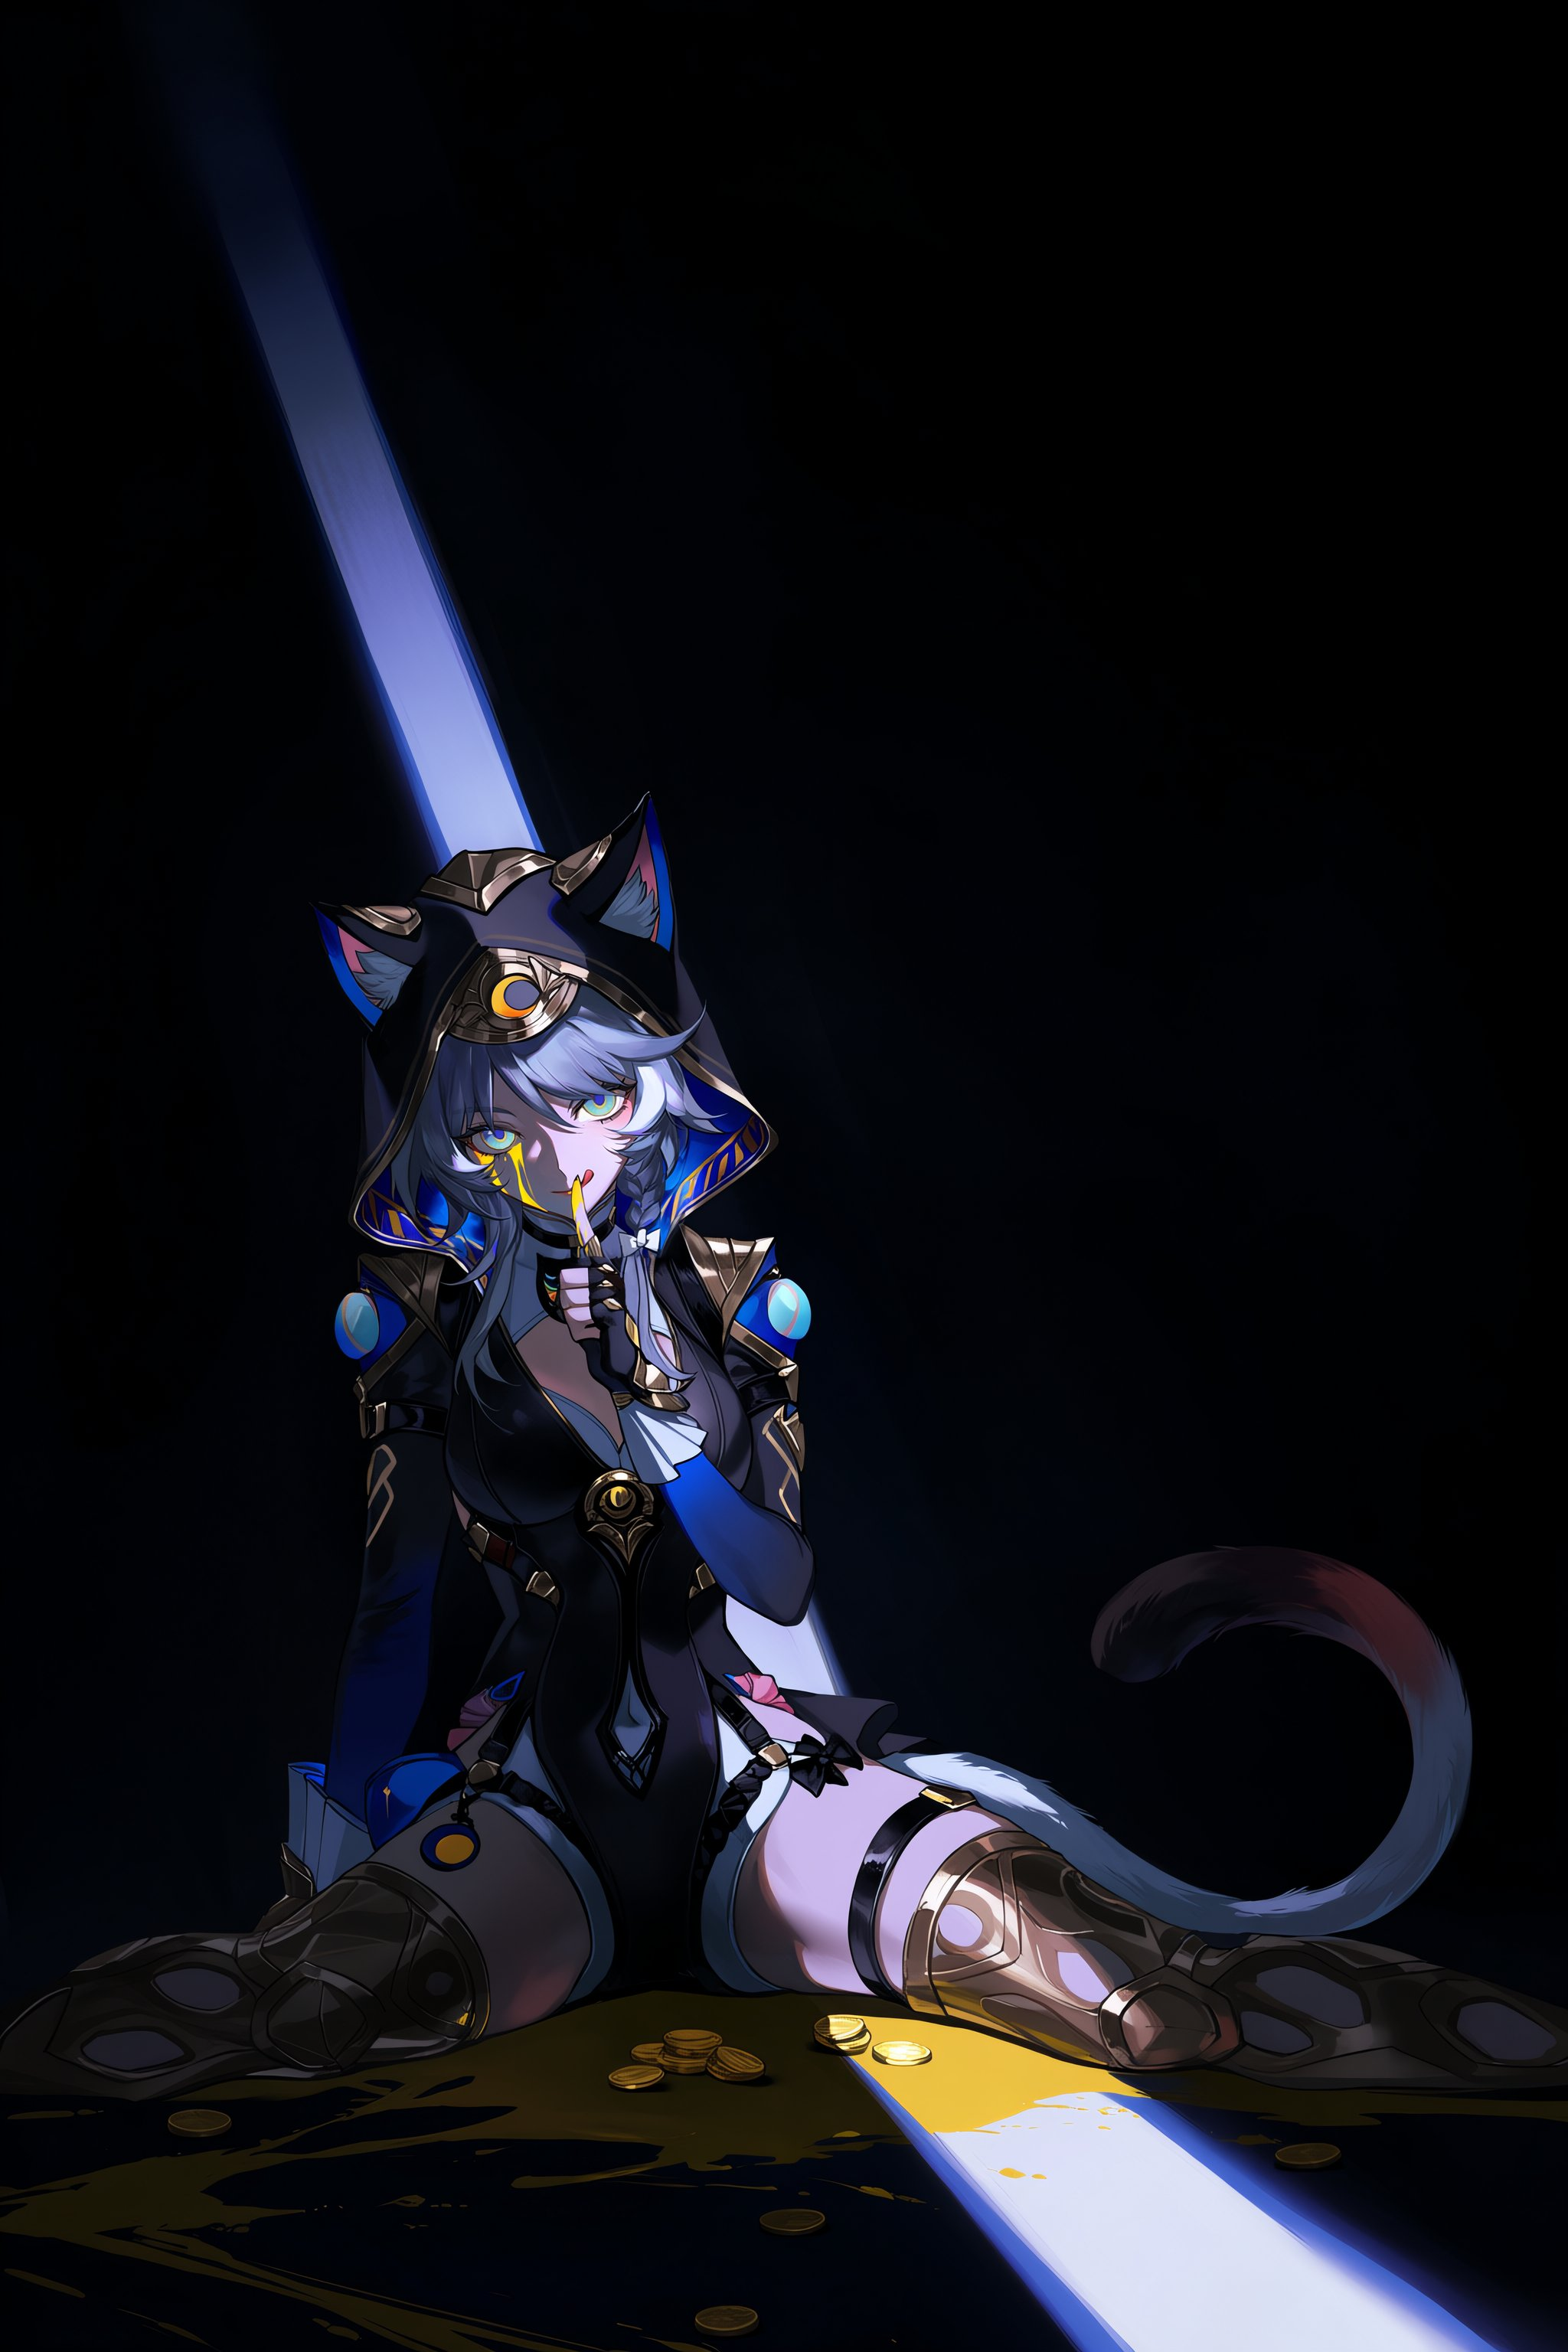
\includegraphics[width=0.632\linewidth]{01705E46-405A-4D35-B256-EFB8333F11DB.JPG}
\end{center}
\newpage
\pagecolor{white}
\color{black}
\tableofcontents
\newpage
\section{Concepts of Computer Science}
\subsection{Computer fundamentals}
\subsubsection{Computer hardware and operation}
\paragraph{Function and interaction of the main CPU components}
The CPU is the critical component that carries out the majority of the processing tasks in a computer system. Consists of:
\begin{itemize}
    \item Control Unit (CU): Directs the operations of the processor. Responsible for the FDE cycle (managing all three operations) + directing the computer's memory, ALU \& I/O devices to carry out the program instructions.
    \item Arithmetic Logic Unit (ALU): Performs arithmetic and logical operations.
    \item Registers: Small, fast storage locations within the CPU that hold data and instructions temporarily during processing.
    \begin{itemize}
        \item Program Counter (PC): Holds the address of the next instruction to be executed.
        \item Memory Address Register (MAR): Holds the address of the memory location that is currently being fetched.
        \item Memory Data Register (MDR): Holds the data that is being transferred to or from memory.
        \item Accumulator (ACC): Holds the result of arithmetic and logical operations performed by the ALU.
        \item Instruction Register (IR): Holds the current instruction being executed.
    \end{itemize}
    \item Buses: Communication pathways that transfer data between the CPU, memory, storage, and I/O devices.
    \begin{itemize}
        \item Data Bus: Transfers data between the CPU, memory, and I/O devices. Bidirectional.
        \item Address Bus: Transfers memory addresses from the CPU to memory. Unidirectional.
        \item Control Bus: Transfers control signals from the CPU to other components. Bidirectional.
    \end{itemize}
\end{itemize}
\textbf{Core:} the processing unit of the CPU. More cores generally means better performance, as multiple cores can handle multiple tasks simultaneously. However, the performance gain depends on the software's ability to utilize multiple cores effectively.\\
Single core processors work well for naturally sequential tasks, while multi-core processors excel in parallel processing tasks.\\
\textbf{Cache:} a small, fast memory located close to the CPU that stores frequently accessed data and instructions. It helps reduce the time it takes for the CPU to access data from main memory. (L1, L2, L3)\\
\textbf{Co-processors:} specialized processors designed to support the main CPU. Tasks from the CPU are offloaded to the co-processor so that they could run in parallel, which can perform them more efficiently. Examples include DSPs, GPUs, and AI accelerators.\\
\textbf{Von Neumann vs Harvard architecture:} Von Neumann architecture uses a single memory space for both instructions and data, while Harvard architecture uses separate memory spaces for instructions and data. Harvard architecture can provide better performance for certain applications, as it allows simultaneous access to both instructions and data. However, it can be more complex to implement and may require more hardware resources.
\paragraph{Role of GPU}
Used to accelerate the rendering of images, videos, and animations. It is particularly effective for tasks that can be parallelized, such as graphics processing and machine learning. 
\begin{itemize}
    \item GPUs have a large number of cores that can handle multiple tasks simultaneously, making them well-suited for tasks that require high computational power.
    \item They also handle the application of shaders and textures to 3D models, which includes lighting, shading and texture mapping. 
    \item GPUs assist in decoding and encoding video streams, which is essential for video playback, video editing, and streaming applications.
    \item Due to the ability to perform parallel processing + matrix and vector operations, GPUs are widely used in machine learning and deep learning applications, where they can accelerate the training and inference of neural networks (esp. for deep learning models).
    \item GPUs also significantly outperformed CPUs in solving cryptographic puzzles, which is why they are widely used in cryptocurrency mining.
\end{itemize} 
\textbf{Accelerators}: separate main circuit board with the processor, memory, power management, etc., but they can not operate by themselves. They are always part of a system (host) in which the CPUs run the operating systems and control the programs execution. (GPU can be one example as well)
\paragraph{Difference between CPU and GPU}
\textbf{Heterogeneous programming}: CPU acts as a main processor, controlling the execution workflow. The host makes all calls, allocates the memory, and handles the memory transfers between CPU and GPU. GPUs run tens of thousands of threads simultaneously on thousands of cores and does not do much of the data management. The device code is executed by doing calls to functions (kernels) written specifically to take advantage of the GPU. \\\\
Overview: The CPU is great for handling various jobs, but the GPU is better for doing the same job many times on a lot of data at once.\\
Usage scenarios:
\begin{itemize}
\item  CPU: Used for general-purpose tasks that require flexibility, quick decisions, and
coordination—such as running an operating system, web browsing, word processing, and managing program instructions.
\item  GPU: Used for tasks involving many similar calculations that can be carried out simultaneously / in parallel, such as rendering graphics in video games, training AI models, machine learning, video editing, and large simulations.
\end{itemize}
\begin{center}
    \begin{tabular}{|p{2.2cm}|p{4.5cm}|p{6.5cm}|p{4.5cm}|}
\hline
\textbf{Processor} & \textbf{Processing} & \textbf{Architecture} & \textbf{Functionality} \\
\hline
CPU & It is a \textbf{general} purpose processor, capable of handling many different tasks. It executes the instructions of computer programs, involving operations such as arithmetic, logic and controlling input / output (I/O) operations, as directed by the operating system. & CPUs generally have fewer cores. Each core is very versatile, making it capable of handling complex computations that require sequential processing. & Allows the user to switch between multiple tasks and applications. This makes it ideal for running the operating system and general software applications. \\
\hline
GPU & It is a \textbf{specialized} processor, with a focus on handling graphics, \textbf{rendering} images, video and animations. & Composed of hundreds or thousands of small cores that are well-suited for tasks that can be run in parallel. While each core is not as powerful as a standard CPU core, the high number of cores allows them to perform a large number of calculations simultaneously, making them perfect for graphical processing. & Suited for tasks that require simultaneous processing of large blocks of data, such as rendering images, video processing and deep learning applications. \\
\hline
\end{tabular}
\end{center}
In case of collaborative efforts to video games operation:
\begin{itemize}
	\item The CPU handles the game’s core logic, including rules, physical calculations and AI behaviour. It processes the inputs from the player.
	\item The GPU renders the game’s visuals. It processes vertex and pixel data to draw images on to the screen, including 3D objects, textures and effects such as lighting and shadows. 
\end{itemize}
\paragraph{Purposes of different types of primary memory}
It directly supports the execution of programs by providing the CPU with fast and flexible access to instructions and data. However, not all primary memory is equal: different types serve distinct purposes, trade-offs, and performance characteristics.
\begin{itemize}
    \item RAM, Random Access Memory: holds instructions and data 
for programs that are currently running. Volatile (loses content when powered off) Directly accessible from CPU. Two types of RAM:
	\begin{itemize}
		\item DRAM: capacitors + transistors (needs to be refreshed)
		\item SRAM: flip flops to store data
	\end{itemize}
    \item ROM, Read-only memory: used for storing instructions that are very rarely modified. (e.g. BIOS: initialize and test the system hardware components on startup, and to load the operating system (OS) software from the secondary memory storage into the RAM) 
    \item Cache (Located within CPU): small, but provides high-speed access to the CPU compared to the RAM. It acts as a buffer between the CPU and the slower RAM, storing frequently used data and instructions. Caches are managed by the cache controller, which uses algorithms like Least Recently Used (LRU) to determine which data to keep or evict.
    \begin{itemize}
        \item L1: located directly on the CPU, making it the fastest type of cache. However, it is also the smallest, often only a few kilobytes in size (32KB to 128KB per core). Each CPU core usually has its own L1 cache:
		\begin{itemize}
			\item L1i to store instructions
			\item L1d to store data
		\end{itemize}
        \item L2: either be on the CPU, or located very near the CPU. L2 cache 
is larger than L1 and can be up to several megabytes in size (256KB to 2MB per core), but slighly slower than L1 cache.
        \item L3: located the furthest from the CPU chip. L3 cache may be shared on multiple-core CPUs. It is the largest of the three, and can be up to tens of megabytes in size (2MB to 64MB shared across all cores). It's also the slowest of all three.
    \end{itemize}
	\item Registers: fastest and smallest type of memory in a computer system. Located directly inside the CPU, they provide temporary storage for data and instructions that the processor is actively using.
\begin{itemize}
\item General-purpose: used to store operands, intermediate results, memory addresses, or anything else the executing program needs.
\item Special-purpose: used by the CPU control unit to manage and coordinate instruction execution. 
\end{itemize}
\end{itemize}
Memory Hierarchy: Register $\Rightarrow$ L1 $\Rightarrow$ L2 $\Rightarrow$ L3 $\Rightarrow$ RAM $\Rightarrow$ Secondary storage.\\\\
\textbf{Cache hit:} data being fetched is located within the cache, reduces retrieval time of data\\
\textbf{Cache miss:} data being fetched is only located within RAM / secondary storage. \\
Types of cache miss:
\begin{itemize}
\item  Compulsory (cold): First-time access to data; it is unavoidable as it is inherent in the first reference to the data.
\item  Capacity: Cache too small to hold all data.
\item  Conflict: Multiple addresses map to the same cache line.
\end{itemize}
The percentage of hit rate determines the efficiency and effectiveness of the cache. Systems with a larger cache size will generally perform better, as well as systems with more intelligent prefetching techniques that can predict which data will be needed soon and load it into cache ahead of time.  
\paragraph{FDE cycle}
\begin{enumerate}
	\item Fetch: The CPU fetches an instruction from the memory. 
	\begin{itemize}
		\item The Program Counter (PC) holds the address of the next instruction to be executed.
		\item This address is copied into the Memory Address Register (MAR).
		\item The address is sent to main memory through the address bus.
		\item The instruction stored at that memory location is sent back to the CPU over the data bus and temporarily held in the Memory Data Register (MDR).
		\item The instruction in the MDR is then transferred to the Current Instruction Register (CIR), where it awaits decoding.
		\item Finally, the PC is incremented so it points to the address of the next instruction.
	\end{itemize}
	\item Decode: The CPU interprets the instruction and prepares the necessary operations to execute it. 
	\begin{itemize}
		\item The CU examines the opcode (the part of the instruction that specifies the operation) and determines what the CPU must do.
\item If the instruction includes operands (addresses or data values), the CU prepares to retrieve them—possibly using the MAR and MDR again for memory access.
\item Internal control signals are generated to direct data movement and select the appropriate ALU operation, register sources, or memory accesses.
	\end{itemize}
	\item Execute: The CPU performs the actions required by the instruction. 
	\begin{itemize}
		\item Arithmetic or logic operations: Data from registers are processed in the ALU, with results stored in the Accumulator (ACC) or another register.
\item Memory operations: The MAR and MDR are used again if data must be read from or written to RAM.
\item Control flow operations: The Program Counter (PC) may be updated.
	\end{itemize}
\end{enumerate}
说老实话，这段IB教科书上写的内容还不如IG时期的教科书，所以我就把去年的拿过来了：
\begin{center}
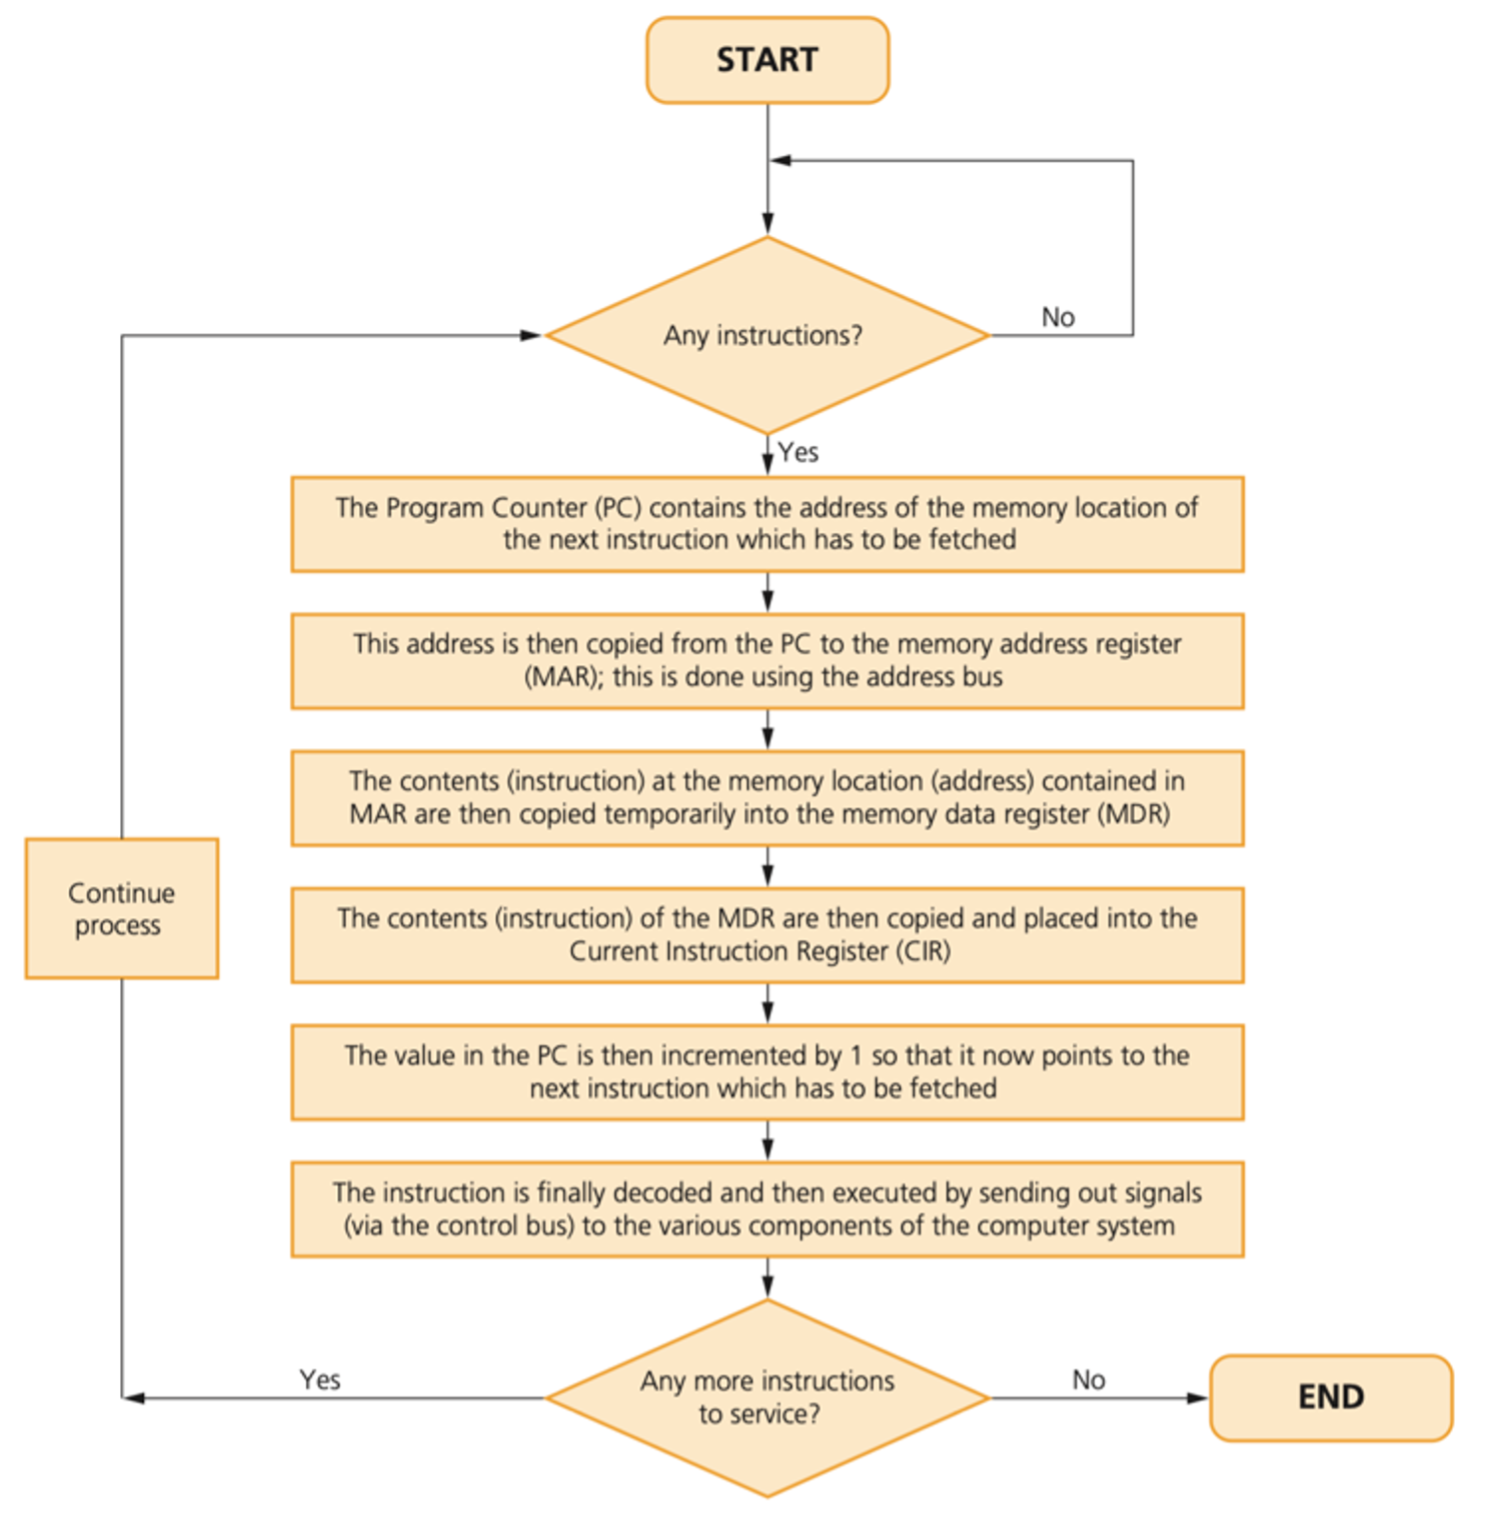
\includegraphics[width=0.9\linewidth]{Picture1.png}
\end{center}
Machine Language: lowest level of programming language that directly corresponds to the instructions executed by a computer's hardware. (In simple terms: binary.)
\paragraph{Pipelining in multi-core architectures}
\paragraph{Internal and external types of secondary memory storage}
\begin{itemize}
	\item Internal Storage
	\begin{itemize}
	\item HDD: utilize a spinning magnetic disk to read / write data. They are suitable for storing large volumes of data, such as media files, backups, and documents, where speed is not so critical. 
	\item SSD: use flash memory to store data, offering high-speed data access and durability. This makes them very popular in portable devices such as laptops and tablets.
	\item eMMC: a type of flash storage that utilizes NAND flash memory. They are soldered directly on to the motherboard of the device. While the capacity and speed do not match a standard SSD, their performance is adequate for basic computing needs and simple applications. 
\end{itemize}
	\item External Storage
\begin{itemize}
\item HDDs \& SSDs: performance and comparison are identical to the internal versions. 
\item Optical discs and optical drives (CD, DVD, blu-rays): cost of an optical disc is low compared to an HDD or SSD and, while their read / write speeds may be slower, they are sufficient for data archiving and playback. However, the discs are prone to scratches, especially if they are not stored correctly, and they require an optical drive to read and write to them.
\item Memory cards (SD, microSD, CF): compact storage devices often used in cameras, smartphones and other portable devices. They are ideal for expanding storage in mobile devices and for storing photos 
and videos in cameras, using NAND flash memory. Highly durable; read / write times are generally slower 
than SSDs, but outperform those of optical discs. 
\item NAS: dedicated file storage connected to a network that allows multiple users to access 
data. It is often used in homes or businesses for centralizing data storage, file storage 
and data backup. Usually made up of multiple HDDs and SSDs configured in RAIDs. It is normally connected to the network via Ethernet, and runs a lightweight operating system designed for file storage, and the management and sharing of files. 
\end{itemize}
\end{itemize}
Comparison between HDDs and SSDs:
\begin{center}
\begin{tabular}{|p{4cm}|p{6.5cm}|p{6.5cm}|}
        \hline
        \textbf{Feature} & \textbf{HDD (hard disk drive)} & \textbf{SSD (solid state drive)} \\
        \hline
        Storage technology & Magnetic storage with spinning disks and read / write heads & Flash memory with no moving parts \\
        \hline
        Speed & Slower read / write speeds (generally 50--150 MB/s) & Faster read / write speeds (generally 200--500 MB/s) \\
        \hline
        Durability & More prone to physical damage due to moving parts & More durable; resistant to physical shock \\
        \hline
        Noise & Produces noise due to moving parts & Silent operation \\
        \hline
        Power consumption & Higher power usage due to mechanical parts & Lower power consumption \\
        \hline
        Cost & Generally cheaper per GB & More expensive per GB \\
        \hline
        Capacity & Available in larger capacities (up to several TB) & Typically available in smaller capacities (up to several TB, but at a higher cost) \\
        \hline
        Weight & Heavier due to mechanical components & Lighter \\
        \hline
        Heat generation & Generates more heat due to moving parts & Generates less heat \\
        \hline
    \end{tabular}
\end{center}

\paragraph{Compression}
\begin{itemize}
\item Lossy: reduces files by permanently eliminating certain information. This information 
is redundant or less critical data, resulting in a compressed version that is not identical 
to the original but is, ideally, indistinguishable from the original to human senses.
\begin{itemize}
\item Transform encoding: 
\begin{center}
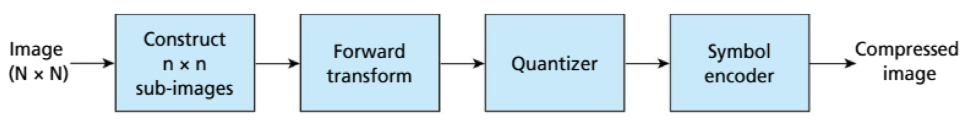
\includegraphics[width=0.8\linewidth]{Screenshot 2026-09-17 at 23.00.02.png}
\end{center}
\begin{enumerate}
\item Transform coding takes an image of N $\times$ N size and sections it into smaller sub-images of size n $\times$ n. 
\item Then the forward transform is carried out on each of the sub-images. The forward transform can use different algorithms, depending on the type of file compression, but for JPEGs DCT (discrete cosine transform) is used. This takes the image data from the spatial domain (pixel values) to the frequency domain. The output breaks the sub-image down into low- and high-frequency coefficients.
\begin{itemize}
\item Low-frequency data: correspond to slow changes in pixel values, such as broad areas. 
\item High-frequency data: correspond to rapid changes in pixel values, representing fine details, edges and textures. 
\end{itemize} 
\item These frequency coetficients are then passed to the quantizer. This step significantly reduces file size by simplifying the frequency coefficients obtained from the DCT. The purpose of quantization is to reduce the precision of high-frequency components (the fine details) rather than low-frequency components. This is because the human eye is less sensitive to high-frequency data loss compared to low-frequency detail. The extent of the quantization decides the compression level and the quality of the final image.
\item The final step of transform coding is the symbol encoder. This is where the quantized coefficients are further compressed using entropy coding techniques. This runs through three further algorithms to reduce the file size by efficiently representing the frequency of occurrence of each symbol. The algorithms used at this stage are 
\begin{enumerate}
\item Zigzag scan
\item RLE
\item Huffman coding
\end{enumerate}
\end{enumerate}
\end{itemize}
\item Lossless: data is compressed to a smaller size, but can be restored back to the original without any loss of information. This technique works by identifying and eliminating statistical redundancy within the data, and this process can be reversed when needed. 
	\begin{itemize}
		\item Run-length encoding: used to reduce the
size of files containing many consecutive repeated characters. The original string of info is represented by the recurrence of the letter + the letter itself. RLE is straightforward to implement and it is very effective for data with lots of repetitions, such as simple graphics and certain types of text file
	\end{itemize}
\end{itemize}
\paragraph{Type of services in cloud implementation}
\begin{itemize}
\item SaaS: delivers software applications over the internet. SaaS provides a cost-effective and convenient solution for businesses and individuals, offering a wide range of applications from productivity tools to customer-relationship management systems. 
\item PaaS: provides a cloud-based platform that allows developers to build, test and deploy applications without managing the underlying infrastructure. PaaS includes tools \& services to facilitate application development, such as databases, middleware (software that connects different applications) and dev frameworks. PaaS accelerates software development by allowing developers to focus on coding rather than infrastructure management.
\item IaaS: provides virtualized computing resources over the internet, such as virtual machines, storage and networks. IaaS gives users full control over their virtual machines and networks. This reduces the need for upfront investment in hardware and allows businesses to rent solutions at a lower initial cost using a subscription model. IaaS is also scalable, making it easy to adjust resources as the user base grows.
\end{itemize}
\subsubsection{Data representation and computer logic}
都是老生常谈的东西，看看就好。金波尔万岁！！！
\paragraph{Principal methods of representing data}
Modern computing ultimately settled on binary (base-2) as the primary number system. The base-2 system represents two possible states: 1 or 0. The binary system is particularly well-suited to represent the state of electrical switches within a computer system: on (1) and off (0). This simplicity reduces hardware complexity and enhances reliability. \\\\
The increased reliability of binary systems stems from their use of only two states. Small 
variations in signal strength do not affect data integrity as much as in systems using larger bases, making binary more robust in noisy (electrical disturbances) environments. 
\[
\begin{array}{|c|c|}
\hline
\textbf{Conversion} & \textbf{Method} \\ \hline

\text{Binary} \rightarrow \text{Decimal}
&
\begin{array}{l}
\text{Multiply each binary digit by its corresponding power of }2,\\
\text{then add the results.}\\
1011_2 = 1(2^3)+0(2^2)+1(2^1)+1(2^0)\\
\phantom{1011_2}=8+0+2+1=11_{10}
\end{array}
\\ \hline

\text{Decimal} \rightarrow \text{Binary}
&
\begin{array}{l}
\text{Repeatedly divide the decimal number by }2,\\
\text{record the remainders, and read them from bottom to top.}\\
\text{I'd personally recommend the subtraction method.}\\
\text{(Subtract the decimal number by powers of 2 and record the results.)}\\
\text{If you use this method, remember to start with the most significant bit (MSB)}\\\text{the left most bit, not the least significant bit (LSB) (which is the right most bit.) }
\end{array}
\\ \hline

\end{array}
\]
Base-2 vs Base-10:
\begin{center}
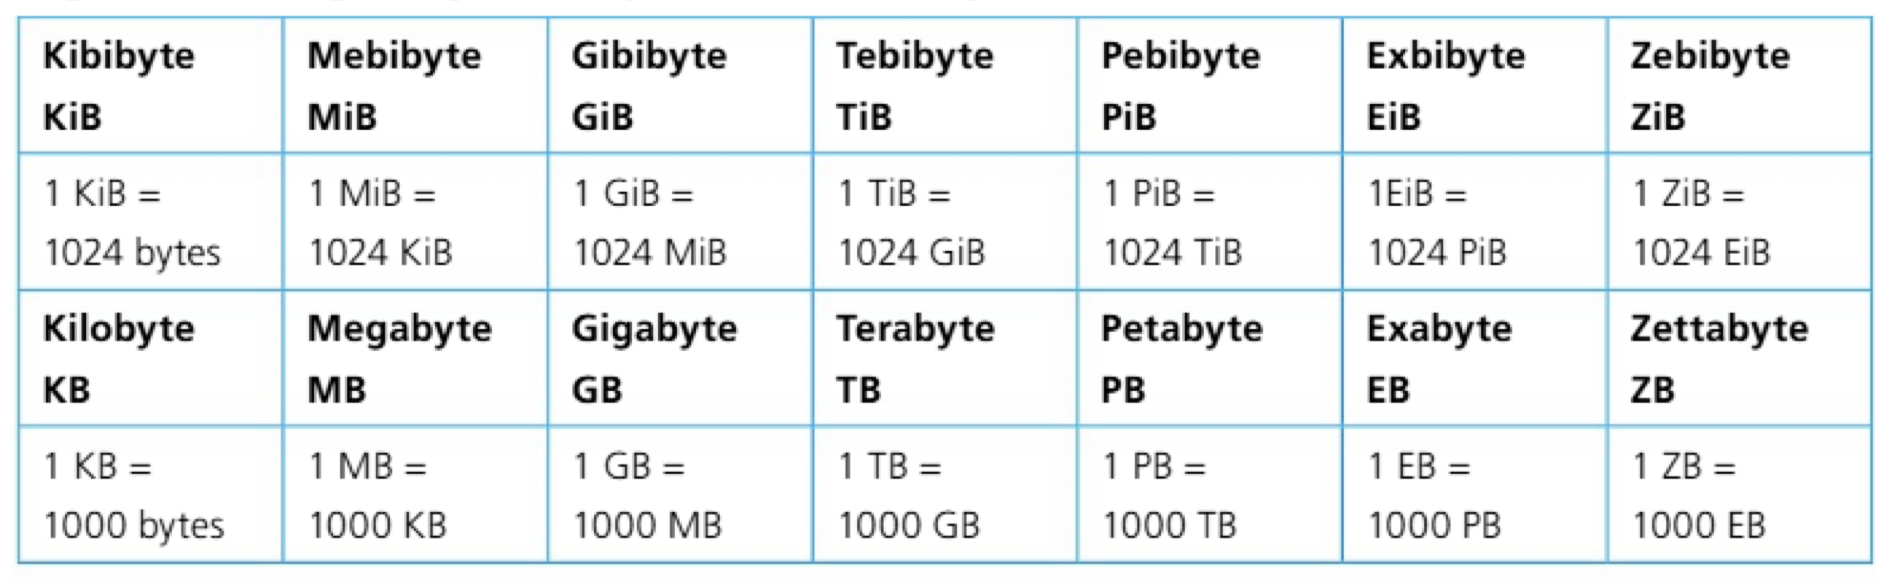
\includegraphics[width=0.9\linewidth]{Screenshot 2026-09-24 at 12.41.11.png}
\end{center}
1 byte = 8 bits, 1 nibble = 4 bits. Note here that KB and Kb are different units. ($KB=8\times Kb$)\\\\
Hexadecimal: base-16 number system, where 10 - 15 are represented by A to F.\\
Reasons for using hexadecimal: 
\begin{itemize}
    \item Ease of conversion between binary and hexadecimal
    \item Compact size of display (used in debugging tools, memory dumps and assembly language programming)
\end{itemize}
Conversion of hexadecimal $\Leftrightarrow$ binary: split the binary in nibbles and turn into hexadecimal for assembling the result. The reverse also stands; i.e. convert each hexadecimal character to binary nibbles, and assemble them in the correct order. (For decimal conversion, I recommend conversion to binary first and then convert to hexadecimal) 
\paragraph{How binary is used to store data}
\begin{itemize}
    \item Characters and strings
    \begin{itemize}
        \item ASCII encoding: designed to provide a common standard for the interchange of text data. Initially started out as 7-bit encoding system (later 8 bits for more character support). Taking the 8-bit system as an example:
\begin{itemize}
    \item $010.....$ represents uppercase letters, while $011.....$ represents lowercase letters.
    \item The last 5 digits, when converted from binary to decimal, corresponds to the alphabet letters (e.g. 1 $\rightarrow$ a, 2 $\rightarrow$ b)
\end{itemize}
	\item Unicode encoding: provides a unique number for every character, regardless of platform, program or language. Few different versions of Unicode:
	\begin{center}
		\renewcommand{\arraystretch}{1.5}
\begin{tabular}{|p{2cm}|p{4cm}|p{5.5cm}|p{4cm}|}
\hline
& \textbf{UTF-8} & \textbf{UTF-16} & \textbf{UTF-32} \\
\hline
\textbf{Variable length encoding} & 1--4 bytes per character & 2 or 4 bytes per character & 4 bytes per character \\
\hline
\textbf{Note} & Compatibility: backward compatible with ASCII & Surrogate pairs: for characters outside the \textbf{Basic Multilingual Plane} (the 
maost commonly used characters and symbals for almost all modern 
languages), two 16-bit code units are used & Simplicity: easier to process because each character is exactly 4 bytes \\
\hline
\textbf{Usage} & Most commonly used encoding on the web and in many applications & Often used in Windows and Java environments & Less common due to higher storage requirements \\
\hline
\end{tabular}
	\end{center}
\item Using UTF-8 as an example: (essentially kept ASCII but added some other bytes in a clever way): 11110000 10011111 10011000 10000100
\begin{itemize}
   \item $11110000$: 1111 means 4 bytes is needed to transmit the character, the 0 coming right after the 4 1s means the end of transmitting the number of bytes. The 3 0s afterwards are the data transmitted.
   \item $10......$: 10 means the continuation bytes being sent, the numbers afterwards are transmitted data.
   \item 0001 1111 0110 0000 0100 are the final data received.
   \end{itemize}
\item UTF-8 has been adopted by the internet as the main character encoding system. Some problems:
\begin{itemize}
    \item Due to the variable length, some characterstake more space compared to single-byte encodings. 
    \item ... This can lead to larger file sizes in certain contexts.
    \item The processing required to handle variable length encoding also requires more complex \\ processing compared to fixed-length 
systems such as UTF-32. 
    \end{itemize}
    \end{itemize}
    \item Images
    \begin{itemize}
        \item Bitmap / raster images: reproduce images by using a grid of pixels, with each pixel assigned a specific colour and intensity. Some key concepts:
        \begin{itemize}
            \item Pixel: short for "picture element", the smallest unit of a digital image / display, representing a single point in the image with a specific color and intensity.
            \item Image resolution: the number of pixels contained within a digital image, typically expressed as the dimensions (width $\times$ height) in pixels, and sometimes as the pixel density (PPI/ DPI) for print quality. 
            \item Color / bit depth: the amount of bits used to describe the color
            \item Formula for calculating image size:
            \[\text{image size (bits) = width}\times \text{height} \times \text{bit depth}\]
However, in reality, this calculation is not completely accurate, as the image would require 
more data to store metadata and other header information.
            \item Metadata: information that describes other data, providing context and details about the data's content, structure and attributes.
        \end{itemize}
		\item Ways to improve the image quality:
		\begin{itemize}
		    \item Increase image resolution. A higher resolution allows for greater detail and clarity. The trade-off for a higher resolution image is larger file size, which can impact storage and transfer efficiency. 依旧老生常谈
		    \item Increase color depth. When we increase the colour depth, it allows for a wider range of colours to be represented, resulting in more vibrant and accurate images. $2^\text{bit depth}=$ numbers of color available for representation. Mostly 24 bits for modern photos.
		\end{itemize}
	\item When working with graphics, RGB values are often shown in hexadecimal. 
    \end{itemize}
    \item Audio: (analog) a continuous signal that represents sound waves through variations of air pressure. These sound waves can be captured through input devices, such as microphones, which convert the sound waves into a digital signal, which is stored as binary. Process: (金波儿老生常谈）
    \begin{enumerate}
        \item An analog to digital converter(ADC) samples the amplitude (loudness) of the sound at discrete intervals in a process known as sampling. The rate at which this happens is measured in Hertz (Hz) — the higher the Hertz, the more samples are recorded per second.
        \begin{itemize}
            \item Amplitude: the magnitude of change in a sound wave, representing the loudness or intensity of the sound. 
            \item  Sampling: the process of converting a continuous analogue signal into a series of discrete digital values by measuring the signal’s amplitude at regular intervals. 
        \end{itemize}
		\item This sample 1s then stored and represented as a numerical value in binary. The precision is determined by the bit depth. The larger the bit depth, the more possible values that can be used to describe the sample.
		\item Formula for calculating audio size:
		\[\text{file size (bits)}=\text{sampling rate}\times \text{bit depth}\times\text{\# of channels}\]
		\item Many formats to choose from for storing audio files: (They mainly differ by whether they are compressed or uncompressed)
		\begin{itemize}
		    \item Uncompressed formats store the raw binary data (e.g. WAV, AIFF)
		    \item Compressed formats use algorithms to reduce the file size for storage or transmission (e.g. MP3, FLAC)
		    \end{itemize}
        \end{enumerate}
    \item Video
    \begin{itemize}
        \item Components include:
        \begin{itemize}
            \item Frames (visual)
            \begin{itemize}
                \item In their raw form, frames are stored the same as images, with each pixel having a value that can be represented using a colour model such as RGB.
                \item To improve colour efficiency, frames are often converted from the RGB colour model to a different one such as YUV. This helps with compression, as this colour model emphasizes luminance (brightness), which the human eye is more sensitive to than changes in colour detail. 
                \end{itemize}
            \item Audio tracks
            \item Metadata
            \item Subtitles and closed captions
            \end{itemize}
			\item Compression methods / techniques
			\begin{itemize}
			    \item Spatial compression: particularly effective and commonly used for video that has significant detail variation in each frame. It reduces file size by eliminating redundant information within each frame, such as colour depth or detail levels.
			    \item Temporal compression: particularly effective and commonly used for video that has consistent motion across frames. It reduces file size by eliminating redundant information between consecutive frames, capturing only the changes or movements from one frame to the next. As a predictive compression technique, it predicts frame content based on the preceding and sometimes following frames, only storing the differences.
			    \end{itemize}
        \end{itemize}
\end{itemize}
Different binary methods for storing integers:
\begin{itemize}
    \item Unsigned binary (covered in A1.2.1)
    \item Signed binary (negative + positive):
    \begin{itemize}
        \item Two's complement: most significant bit represents sign. 0 for positive, 1 for negative. To convert a positive binary number to its negative counterpart in two’s complement, you first invert all the bits and then add 1 to the least significant bit.
        \item One’s complement: To obtain the one’s complement of a positive number, you simply invert all the bits (change 0s to 1s and 1s to 0s). One's complement have TWO (positive and negative) zeros.
        \item Sign-magnitude: most significant bit serves for sign; the remaining bits represent the magnitude of the number, like how unsigned binary numbers work. 
        \end{itemize}
\item Binary-coded decimal: method of representing decimal numbers where each digit of the decimal number is encoded separately into its own binary form. BCD assigns a 4-bit binary code to each decimal digit (0-9). 
\item Gray code (reflected binary code): a binary system where two successive values are only allowed to differ by one bit.
\begin{center}
\begin{tabular}{|c|c|c|}
\hline
\textbf{Decimal} & \textbf{3-bit binary} & \textbf{3-bit Gray code} \\
\hline
0 & 000 & 000 \\
1 & 001 & 001 \\
2 & 010 & 011 \\
3 & 011 & 010 \\
4 & 100 & 110 \\
5 & 101 & 111 \\
6 & 110 & 101 \\
7 & 111 & 100 \\
\hline
\end{tabular}
\end{center}
For example, from decimal 3 to 4, ordinary binary changes from 011 to 100 (three bits change), while Gray code changes from 010 to 110 (only one bit changes).
\item Excess-N (biased representation): a fixed bias (N) is added to the actual value to form an encoded value, and you subtract this bias to decode it. This is used to make all signed integers appear as non-negative binary numbers to allow for easier comparisons and arithmetic operations. 我打算法题的时候有一次这么干过XD
\item Fixed-point representation: a method used to store real numbers (numbers with fractional parts) in binary by fixing the position of the binary point. In a fixed-point system, the binary point is placed at a predetermined position, either between certain bits or at a specific location in the binary sequence. This allows for a straightforward representation of fractional numbers, though with some trade-offs in terms of precision and range.
\item Floating-point representation: a method used to represent real numbers that can have a very large range or fractional parts. It does this by storing numbers in a format that includes a sign, an exponent and a mantissa (or significand).
\begin{enumerate}
    \item Sign bit (one bit): The sign bit determines whether the number is positive or negative. 
    \item Exponent (eight bits): 
This is used to scale the number by a power of two and is stored using the Excess-127 system in its “biased” form.
\item Mantissa (23 bits): 
This represents the significant digits of the number. The mantissa does not store leading ones (in normalized form, $1.xxxxxx\times 2^n$). 
\end{enumerate}
An example of FP representation (32-bit single precision): represent $13.25_{10}$.
\begin{enumerate}
    \item Convert to binary and normalize:
    \[
    13.25_{10} = 1101.01_2 = 1.10101_2 \times 2^3.
    \]
    \item Sign bit: the number is positive, so the sign bit is \texttt{0}.
    \item Exponent: add the bias of 127 to the actual exponent, giving $3 + 127 = 130_{10} = 10000010_2$.
    \item Mantissa: omit the implicit leading 1 and store the fractional bits \texttt{10101}, padded with zeros to 23 bits: \texttt{10101000000000000000000}.
\end{enumerate}
The stored representation is:
\[
\underbrace{\texttt{0}}_{\text{Sign (1 bit)}}\;\vert\;
\underbrace{\texttt{10000010}}_{\text{Exponent (8 bits)}}\;\vert\;
\underbrace{\texttt{10101000000000000000000}}_{\text{Mantissa (23 bits)}}.
\]
To decode it, subtract the exponent bias and restore the implicit leading 1:
\[
(-1)^0 \times (1 + 2^{-1} + 2^{-3} + 2^{-5}) \times 2^{130-127}
= 1.65625 \times 8 = 13.25.
\]
\end{itemize}
\paragraph{Purpose and use of logic gates}
Logic gates are made up of transistors, which act as electronic switches, allowing or blocking the flow of electrical current. In a transistor, the control wire (or “gate”) regulates the current between the two electrodes, known as the “source” and the “drain”. When voltage is applied to the gate, it allows current to flow from the source to the drain, enabling the transistor to switch states and perform logical operations.
\begin{center}

\renewcommand{\arraystretch}{1.15}
\setlength{\tabcolsep}{8pt}

% =========================
% AND
% =========================
\begin{minipage}{0.22\textwidth}
\centering
\begin{circuitikz}
    \node[and port] (G) {};
    \draw (G.in 1) -- ++(-0.6,0);
    \draw (G.in 2) -- ++(-0.6,0);
    \draw (G.out) -- ++(0.6,0);
\end{circuitikz}
\vspace{3mm}

\textbf{AND}

$Y = A \cdot B$

\[
\begin{array}{cc|c}
A & B & Y \\ \hline
0 & 0 & 0 \\
0 & 1 & 0 \\
1 & 0 & 0 \\
1 & 1 & 1
\end{array}
\]

\vspace{2mm}

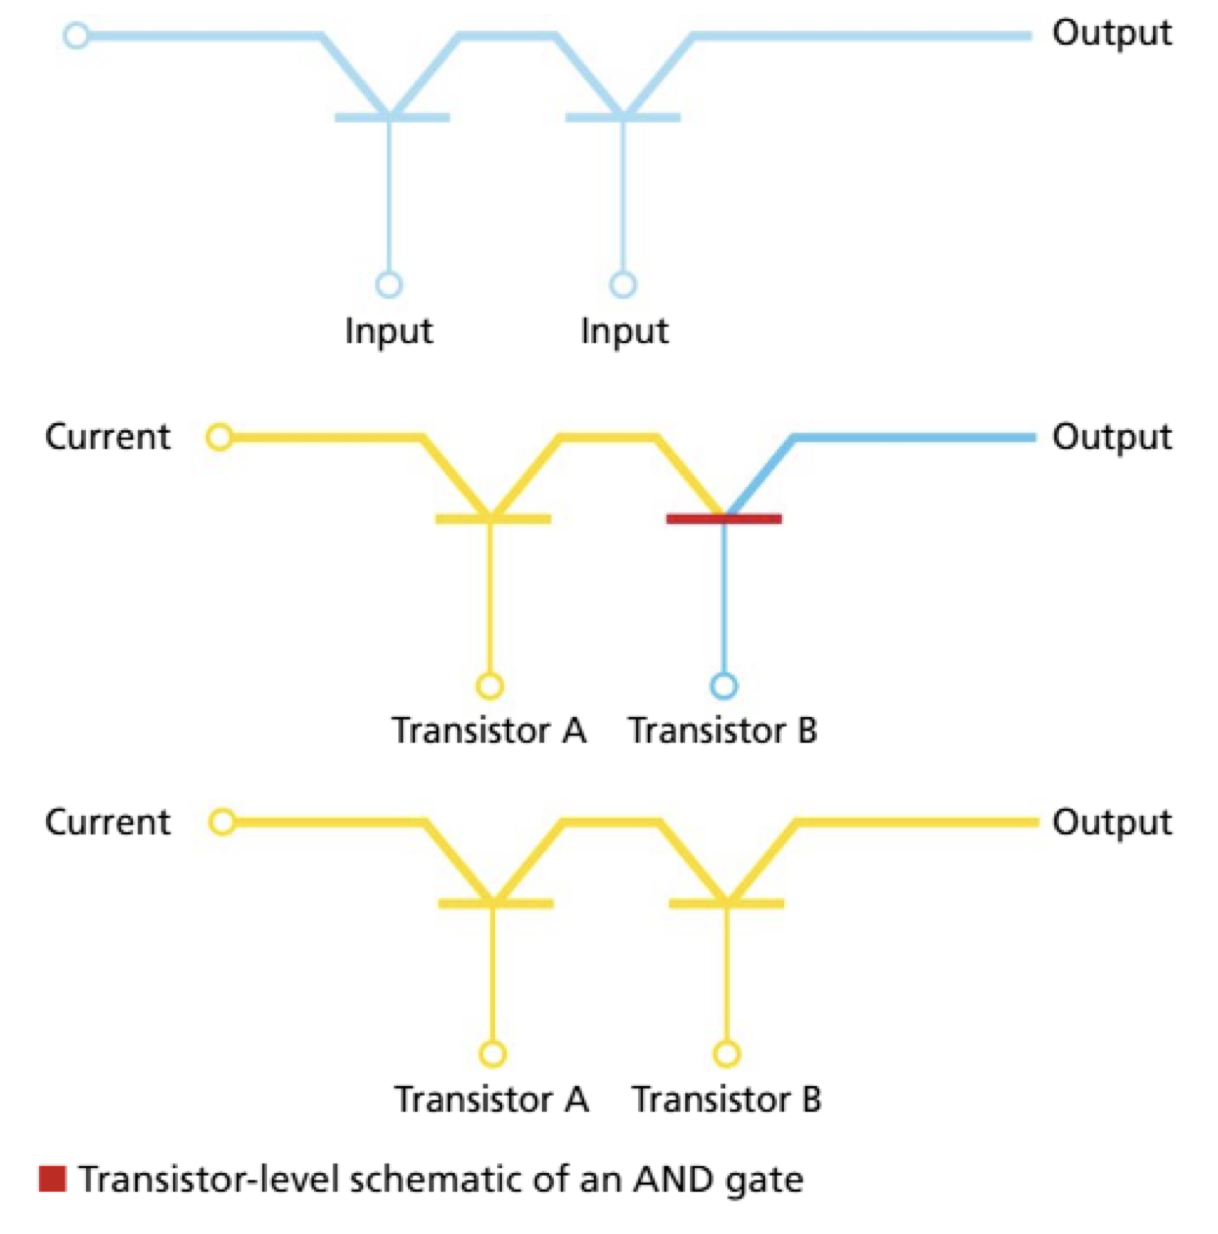
\includegraphics[width=\linewidth]{Screenshot 2026-10-05 at 12.33.38.png}

\end{minipage}
\hfill
% =========================
% OR
% =========================
\begin{minipage}{0.22\textwidth}
\centering
\begin{circuitikz}
    \node[or port] (G) {};
    \draw (G.in 1) -- ++(-0.6,0);
    \draw (G.in 2) -- ++(-0.6,0);
    \draw (G.out) -- ++(0.6,0);
\end{circuitikz}

\vspace{3mm}

\textbf{OR}

$Y = A + B$

\[
\begin{array}{cc|c}
A & B & Y \\ \hline
0 & 0 & 0 \\
0 & 1 & 1 \\
1 & 0 & 1 \\
1 & 1 & 1
\end{array}
\]

\vspace{2mm}

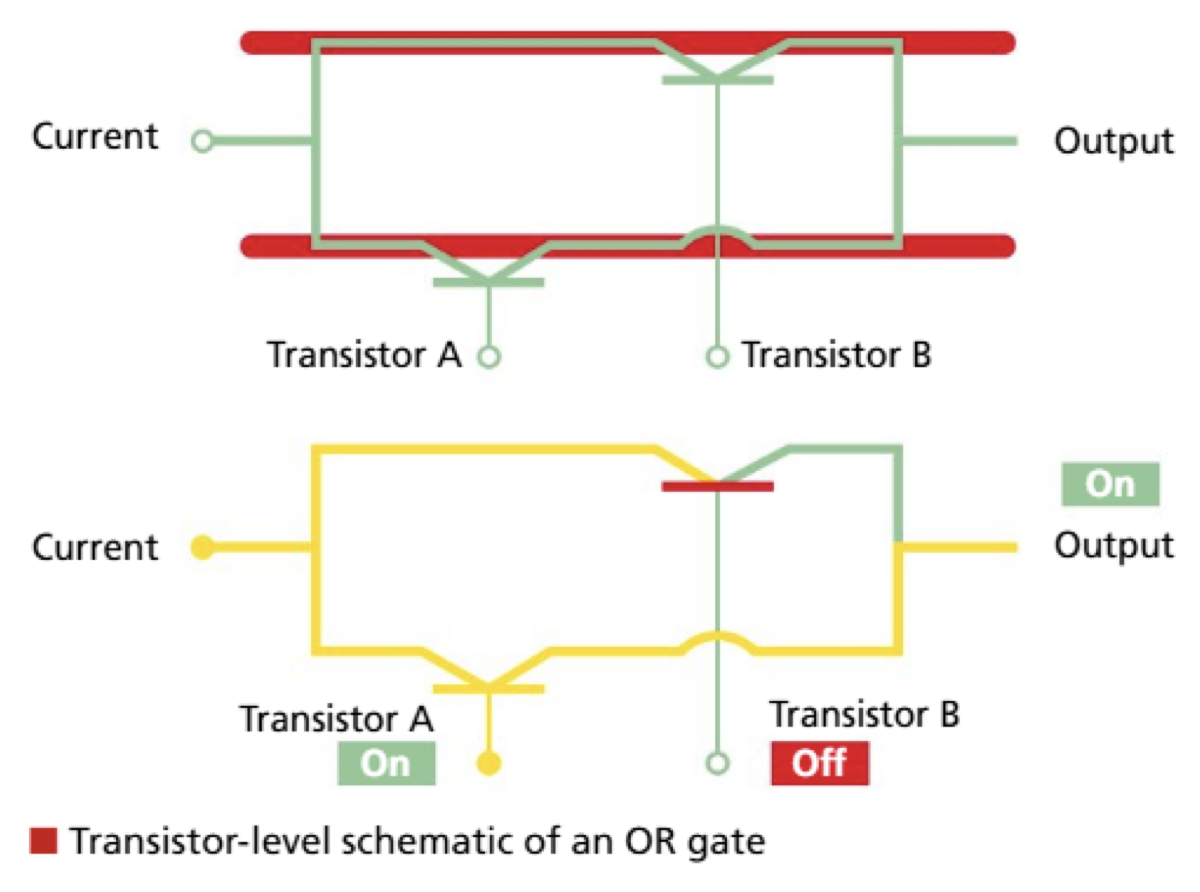
\includegraphics[width=\linewidth]{Screenshot 2026-10-05 at 12.34.03.png}

\end{minipage}
\hfill
% =========================
% NOT
% =========================
\begin{minipage}{0.22\textwidth}
\centering
\begin{circuitikz}
    \node[not port] (G) {};
    \draw (G.in) -- ++(-0.6,0);
    \draw (G.out) -- ++(0.6,0);
\end{circuitikz}

\vspace{3mm}

\textbf{NOT}

$Y = \overline{A}$

\[
\begin{array}{c|c}
A & Y \\ \hline
0 & 1 \\
1 & 0
\end{array}
\]

\vspace{2mm}

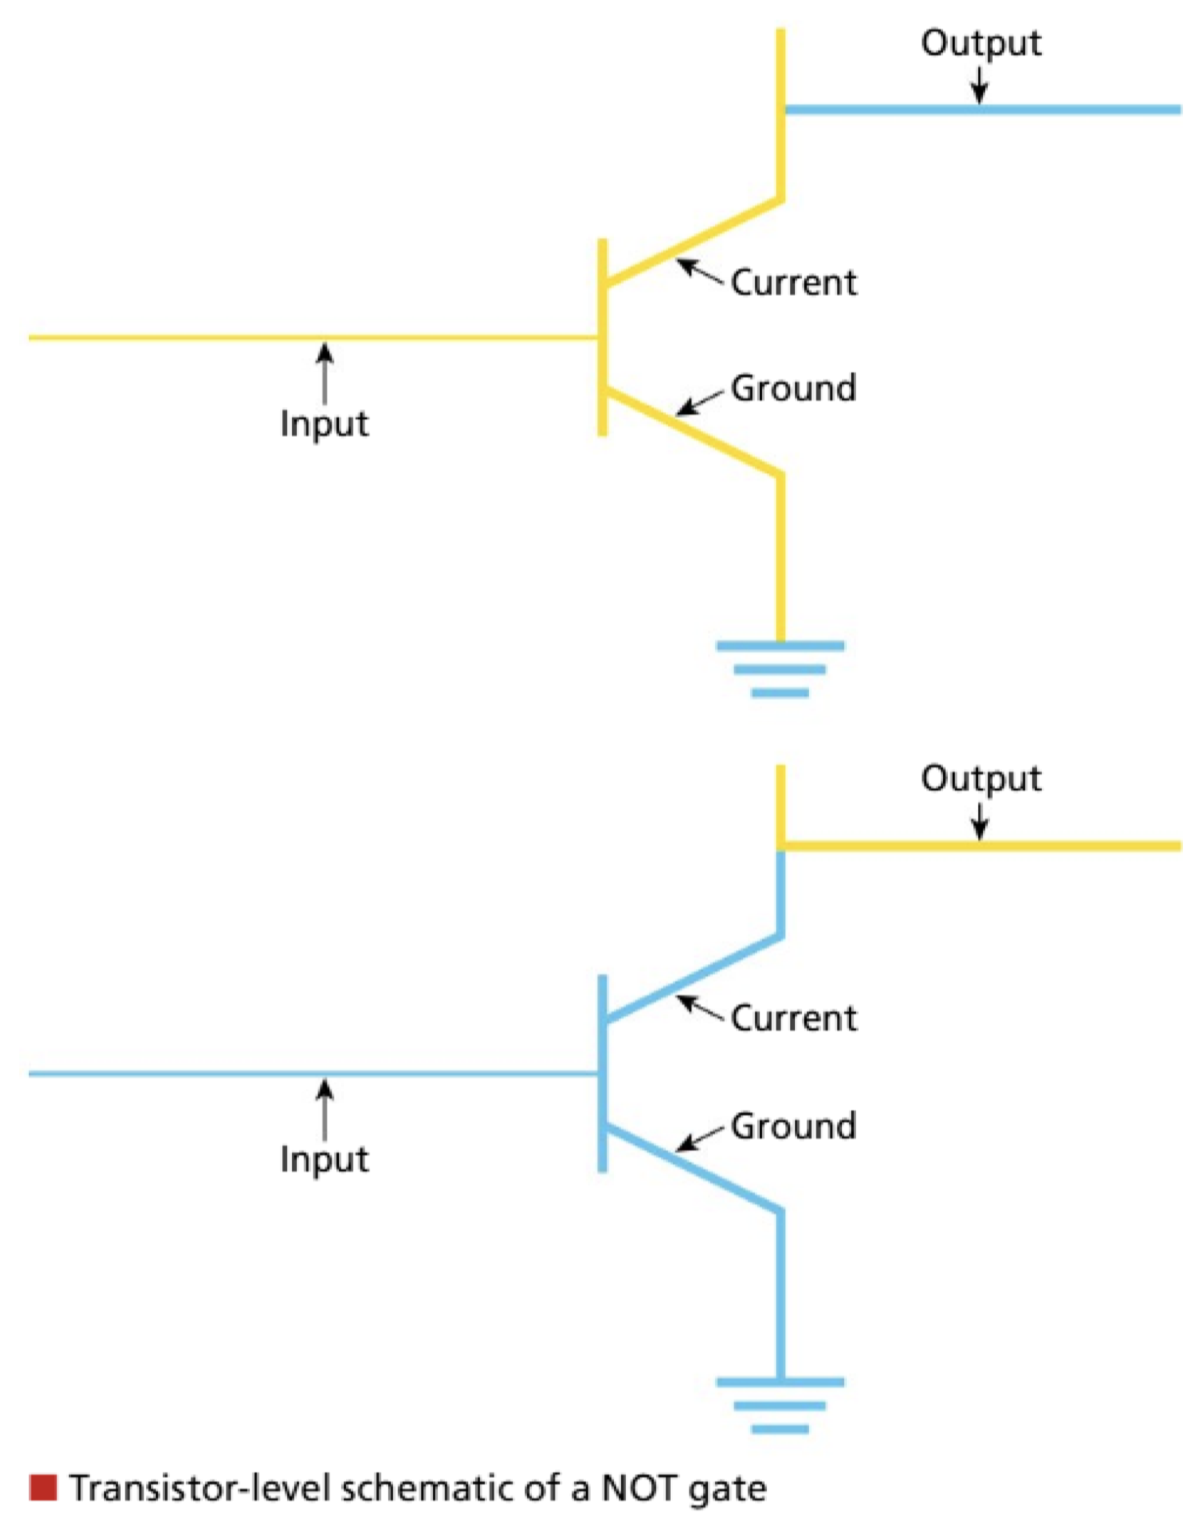
\includegraphics[width=\linewidth]{Screenshot 2026-10-05 at 12.37.18.png}

\end{minipage}
\hfill
% =========================
% BUFFER
% =========================
\begin{minipage}{0.22\textwidth}
\centering
\begin{circuitikz}
    \node[buffer port] (G) {};
    \draw (G.in) -- ++(-0.6,0);
    \draw (G.out) -- ++(0.6,0);
\end{circuitikz}

\vspace{3mm}

\textbf{BUFFER}

$Y = A$

\[
\begin{array}{c|c}
A & Y \\ \hline
0 & 0 \\
1 & 1
\end{array}
\]

\vspace{2mm}

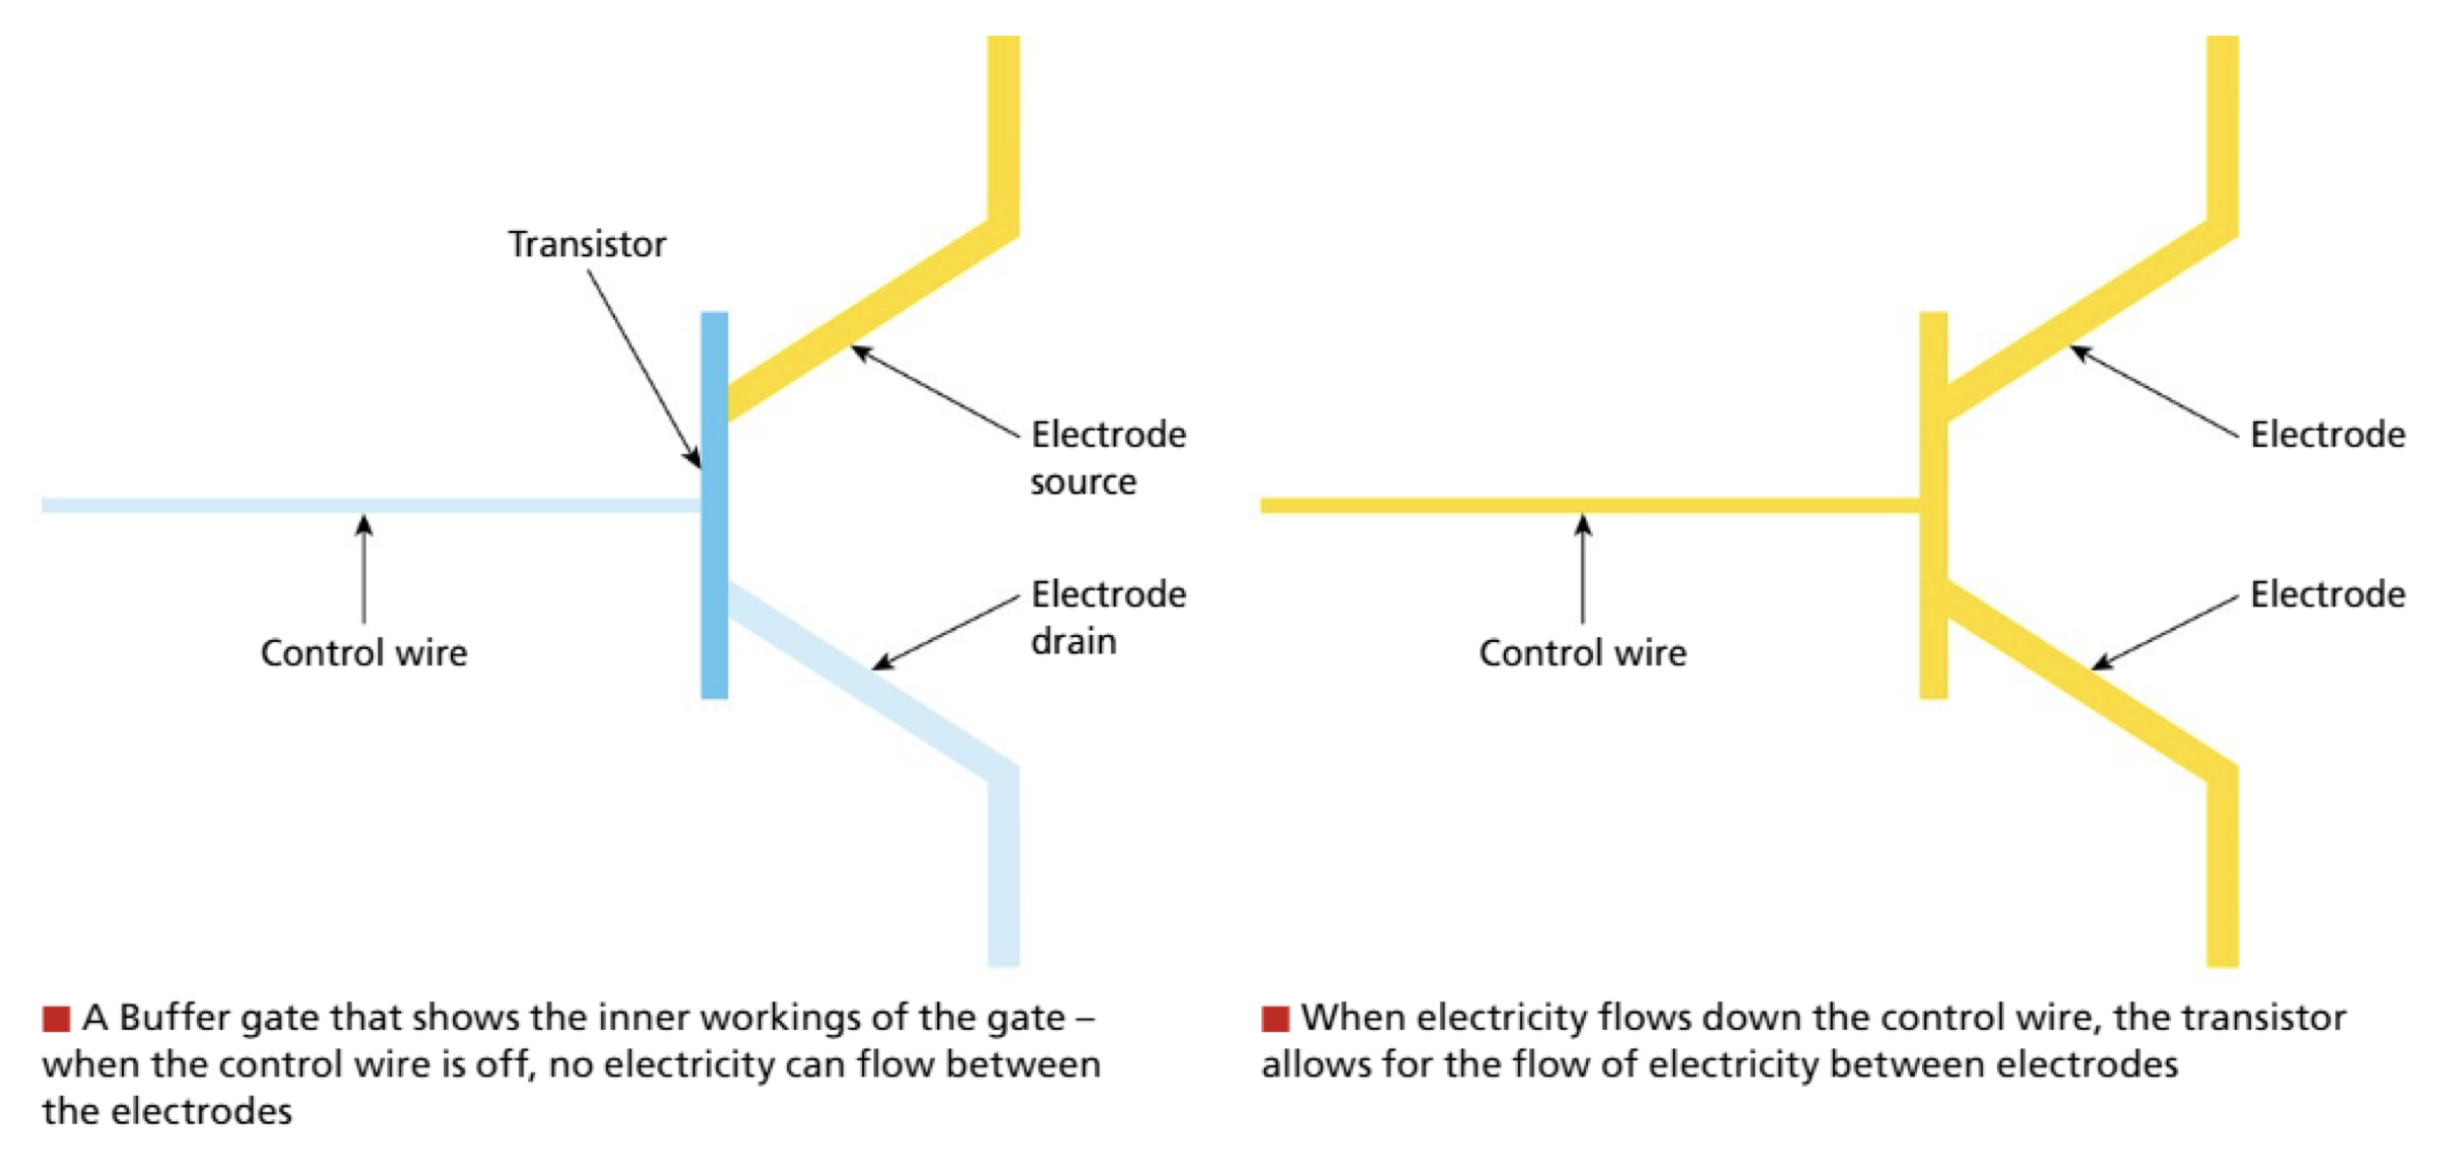
\includegraphics[width=\linewidth]{Screenshot 2026-10-05 at 12.32.29.png}

\end{minipage}

\vspace{12mm}

% =========================
% NAND
% =========================
\begin{minipage}{0.22\textwidth}
\centering
\begin{circuitikz}
    \node[nand port] (G) {};
    \draw (G.in 1) -- ++(-0.6,0);
    \draw (G.in 2) -- ++(-0.6,0);
    \draw (G.out) -- ++(0.6,0);
\end{circuitikz}

\vspace{3mm}

\textbf{NAND}

$Y = \overline{A \cdot B}$

\[
\begin{array}{cc|c}
A & B & Y \\ \hline
0 & 0 & 1 \\
0 & 1 & 1 \\
1 & 0 & 1 \\
1 & 1 & 0
\end{array}
\]

\end{minipage}
\hfill
% =========================
% NOR
% =========================
\begin{minipage}{0.22\textwidth}
\centering
\begin{circuitikz}
    \node[nor port] (G) {};
    \draw (G.in 1) -- ++(-0.6,0);
    \draw (G.in 2) -- ++(-0.6,0);
    \draw (G.out) -- ++(0.6,0);
\end{circuitikz}

\vspace{3mm}

\textbf{NOR}

$Y = \overline{A + B}$

\[
\begin{array}{cc|c}
A & B & Y \\ \hline
0 & 0 & 1 \\
0 & 1 & 0 \\
1 & 0 & 0 \\
1 & 1 & 0
\end{array}
\]

\end{minipage}
\hfill
% =========================
% XOR
% =========================
\begin{minipage}{0.22\textwidth}
\centering
\begin{circuitikz}
    \node[xor port] (G) {};
    \draw (G.in 1) -- ++(-0.6,0);
    \draw (G.in 2) -- ++(-0.6,0);
    \draw (G.out) -- ++(0.6,0);
\end{circuitikz}

\vspace{3mm}

\textbf{XOR}

$Y = A \oplus B$

\[
\begin{array}{cc|c}
A & B & Y \\ \hline
0 & 0 & 0 \\
0 & 1 & 1 \\
1 & 0 & 1 \\
1 & 1 & 0
\end{array}
\]

\end{minipage}
\hfill
% =========================
% XNOR
% =========================
\begin{minipage}{0.22\textwidth}
\centering
\begin{circuitikz}
    \node[xnor port] (G) {};
    \draw (G.in 1) -- ++(-0.6,0);
    \draw (G.in 2) -- ++(-0.6,0);
    \draw (G.out) -- ++(0.6,0);
\end{circuitikz}

\vspace{3mm}

\textbf{XNOR}

$Y = \overline{A \oplus B}$

\[
\begin{array}{cc|c}
A & B & Y \\ \hline
0 & 0 & 1 \\
0 & 1 & 0 \\
1 & 0 & 0 \\
1 & 1 & 1
\end{array}
\]

\end{minipage}

\end{center}

\paragraph{Constructing and analysing truth tables}
Starting with the intermediate values, work through the logic circuit. \\
Number of rows in truth table: $2^\text{\# of inputs}$\\
\textbf{Worked example: four inputs, all eight gate types.}\\
Each gate output is labelled; every label becomes a column of the truth table.
\[
\begin{aligned}
T_1 &= \operatorname{BUF}(A) = A &&\text{(BUFFER)}\\
T_2 &= \overline{T_1} = \overline{A} &&\text{(NOT)}\\
T_3 &= T_2 \cdot B = \overline{A}\,B &&\text{(AND)}\\
T_4 &= T_3 + C = \overline{A}\,B + C &&\text{(OR)}\\
T_5 &= T_4 \oplus D = (\overline{A}\,B + C)\oplus D &&\text{(XOR)}\\
T_6 &= \overline{T_5 \cdot B} &&\text{(NAND)}\\
T_7 &= \overline{T_6 + C} &&\text{(NOR)}\\
Y   &= \overline{T_7 \oplus D} &&\text{(XNOR)}
\end{aligned}
\]
Standard gate operators
$X\uparrow Y=\overline{X\cdot Y}$ (NAND), $X\downarrow Y=\overline{X+Y}$ (NOR)
and $X\odot Y=\overline{X\oplus Y}$ (XNOR),
\[
Y=\Big(\big(((\overline{A}\cdot B)+C)\oplus D\big)\uparrow B\Big)\downarrow C\ \odot\ D .
\]
\begin{center}
\resizebox{0.99\linewidth}{!}{%
\begin{tikzpicture}
% ---- gates ----
\node[buffer port] (T1) at (0,0) {};
\node[not port]    (T2) at (1.8,0) {};
\node[and port]    (T3) at (4.2,0) {};
\node[or port]     (T4) at (6.6,0) {};
\node[xor port]    (T5) at (9.0,0) {};
\node[nand port]   (T6) at (11.4,0) {};
\node[nor port]    (T7) at (13.8,0) {};
\node[xnor port]   (TY) at (16.2,0) {};
% ---- input taps above (B, C and D buses) ----
\draw (-1.5,2.2) -- (9.714,2.2);
\draw (2.514,2.2) -- (2.514,0.28) -- (2.814,0.28);
\draw (9.714,2.2) -- (9.714,0.28) -- (10.014,0.28);
\fill (2.514,2.2) circle (0.045);
\draw (-1.5,3.2) -- (12.114,3.2);
\draw (4.914,3.2) -- (4.914,0.28) -- (5.214,0.28);
\draw (12.114,3.2) -- (12.114,0.28) -- (12.414,0.28);
\fill (4.914,3.2) circle (0.045);
\draw (-1.5,4.2) -- (14.514,4.2);
\draw (7.314,4.2) -- (7.314,0.28) -- (7.614,0.28);
\draw (14.514,4.2) -- (14.514,0.28) -- (14.814,0.28);
\fill (7.314,4.2) circle (0.045);
% ---- input A ----
\draw (-1.5,0) -- (T1.in);
\node[left] at (-1.5,0) {$A$};
\node[left] at (-1.5,2.2) {$B$};
\node[left] at (-1.5,3.2) {$C$};
\node[left] at (-1.5,4.2) {$D$};
% ---- signal chain ----
\draw (T1.out) -- (T2.in);
\draw (T2.out) -- (2.814,0) -- (T3.in 2);
\draw (T3.out) -- (5.214,0) -- (T4.in 2);
\draw (T4.out) -- (7.614,0) -- (T5.in 2);
\draw (T5.out) -- (10.014,0) -- (T6.in 2);
\draw (T6.out) -- (12.414,0) -- (T7.in 2);
\draw (T7.out) -- (14.814,0) -- (TY.in 2);
\draw (TY.out) -- (17.1,0) node[right] {$Y$};
% ---- labels ----
\node[above=1pt] at (T1.north) {$T_1$};
\node[above=1pt] at (T2.north) {$T_2$};
\node[above=1pt] at (T3.north) {$T_3$};
\node[above=1pt] at (T4.north) {$T_4$};
\node[above=1pt] at (T5.north) {$T_5$};
\node[above=1pt] at (T6.north) {$T_6$};
\node[above=1pt] at (T7.north) {$T_7$};
\node[below=1pt] at (T1.south) {\scriptsize BUF};
\node[below=1pt] at (T2.south) {\scriptsize NOT};
\node[below=1pt] at (T3.south) {\scriptsize AND};
\node[below=1pt] at (T4.south) {\scriptsize OR};
\node[below=1pt] at (T5.south) {\scriptsize XOR};
\node[below=1pt] at (T6.south) {\scriptsize NAND};
\node[below=1pt] at (T7.south) {\scriptsize NOR};
\node[below=1pt] at (TY.south) {\scriptsize XNOR};
\end{tikzpicture}}
\end{center}
\begin{center}
\renewcommand{\arraystretch}{1.12}
\begin{tabular}{cccc|ccccccc|c}
\toprule
\multicolumn{4}{c|}{Inputs} & \multicolumn{7}{c|}{Intermediate values} & Output \\
\cmidrule(lr){1-4}\cmidrule(lr){5-11}\cmidrule(lr){12-12}
$A$ & $B$ & $C$ & $D$ & $T_1$ & $T_2$ & $T_3$ & $T_4$ & $T_5$ & $T_6$ & $T_7$ & $Y$ \\
{\scriptsize} & {\scriptsize} & {\scriptsize} & {\scriptsize} & \scriptsize BUF & \scriptsize NOT & \scriptsize AND & \scriptsize OR & \scriptsize XOR & \scriptsize NAND & \scriptsize NOR & \scriptsize XNOR \\
\midrule
0 & 0 & 0 & 0 & 0 & 1 & 0 & 0 & 0 & 1 & 0 & 1 \\
0 & 0 & 0 & 1 & 0 & 1 & 0 & 0 & 1 & 1 & 0 & 0 \\
0 & 0 & 1 & 0 & 0 & 1 & 0 & 1 & 1 & 1 & 0 & 1 \\
0 & 0 & 1 & 1 & 0 & 1 & 0 & 1 & 0 & 1 & 0 & 0 \\
0 & 1 & 0 & 0 & 0 & 1 & 1 & 1 & 1 & 0 & 1 & 0 \\
0 & 1 & 0 & 1 & 0 & 1 & 1 & 1 & 0 & 1 & 0 & 0 \\
0 & 1 & 1 & 0 & 0 & 1 & 1 & 1 & 1 & 0 & 0 & 1 \\
0 & 1 & 1 & 1 & 0 & 1 & 1 & 1 & 0 & 1 & 0 & 0 \\
1 & 0 & 0 & 0 & 1 & 0 & 0 & 0 & 0 & 1 & 0 & 1 \\
1 & 0 & 0 & 1 & 1 & 0 & 0 & 0 & 1 & 1 & 0 & 0 \\
1 & 0 & 1 & 0 & 1 & 0 & 0 & 1 & 1 & 1 & 0 & 1 \\
1 & 0 & 1 & 1 & 1 & 0 & 0 & 1 & 0 & 1 & 0 & 0 \\
1 & 1 & 0 & 0 & 1 & 0 & 0 & 0 & 0 & 1 & 0 & 1 \\
1 & 1 & 0 & 1 & 1 & 0 & 0 & 0 & 1 & 0 & 1 & 1 \\
1 & 1 & 1 & 0 & 1 & 0 & 0 & 1 & 1 & 0 & 0 & 1 \\
1 & 1 & 1 & 1 & 1 & 0 & 0 & 1 & 0 & 1 & 0 & 0 \\
\bottomrule
\end{tabular}
\end{center}
Truth tables to determine outputs from inputs for a problem description: With a problem description, we first need to identify the inputs. Here we have three: alarm switch, baby crying and room temperature, which we can represent as A, B and C and set up our truth table. \\\\
Logical expressions: We can represent logic circuits using Boolean algebra. In Boolean algebra, parentheses are often used to indicate which operations should be 
performed first. If no parentheses are present, follow this sequence: NOT, AND, OR.\\\\
\textbf{Karnaugh maps and algebraic simplification}\\
Two input K-map: the four cells hold the output for the four possible combinations of $A$ and $B$. For example, the function $F=A+B$ gives
\begin{center}
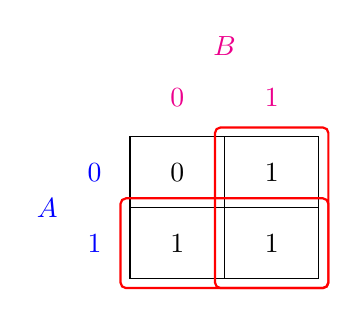
\begin{tikzpicture}[font=\normalsize]
  \draw (0,0) rectangle (2.4,-1.8);
  \draw (1.2,0) -- (1.2,-1.8);
  \draw (0,-0.9) -- (2.4,-0.9);
  \node at (0.6,-0.45) {0};
  \node at (1.8,-0.45) {1};
  \node at (0.6,-1.35) {1};
  \node at (1.8,-1.35) {1};
  \node[text=magenta] at (0.6,0.5) {0};
  \node[text=magenta] at (1.8,0.5) {1};
  \node[text=magenta] at (1.2,1.15) {$B$};
  \node[text=blue] at (-0.45,-0.45) {0};
  \node[text=blue] at (-0.45,-1.35) {1};
  \node[text=blue] at (-1.05,-0.9) {$A$};
  \draw[red, thick, rounded corners=2pt] (1.08,0.12) rectangle (2.52,-1.92);
  \draw[red, thick, rounded corners=2pt] (-0.12,-0.78) rectangle (2.52,-1.92);
\end{tikzpicture}
\end{center}
The two 1s in the column $B=1$ group to give $B$, and the two 1s in the row $A=1$ group to give $A$, so the K-map simplifies to $F=A+B$.\\\\
Three input K-map: the eight cells hold the output for the eight combinations of $A$, $B$ and $C$, with the column labels in Gray-code order $00,01,11,10$ so that adjacent cells differ by one variable. For example, the function $F=AB+C$ gives
\begin{center}
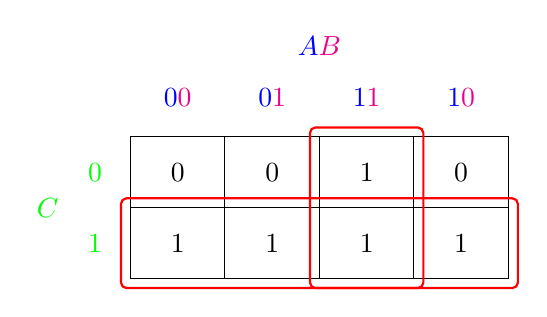
\begin{tikzpicture}[font=\normalsize]
  \draw (0,0) rectangle (4.8,-1.8);
  \draw (1.2,0) -- (1.2,-1.8);
  \draw (2.4,0) -- (2.4,-1.8);
  \draw (3.6,0) -- (3.6,-1.8);
  \draw (0,-0.9) -- (4.8,-0.9);
  \node at (0.6,-0.45) {0};
  \node at (1.8,-0.45) {0};
  \node at (3.0,-0.45) {1};
  \node at (4.2,-0.45) {0};
  \node at (0.6,-1.35) {1};
  \node at (1.8,-1.35) {1};
  \node at (3.0,-1.35) {1};
  \node at (4.2,-1.35) {1};
  \node at (0.6,0.5) {\textcolor{blue}{0}\textcolor{magenta}{0}};
  \node at (1.8,0.5) {\textcolor{blue}{0}\textcolor{magenta}{1}};
  \node at (3.0,0.5) {\textcolor{blue}{1}\textcolor{magenta}{1}};
  \node at (4.2,0.5) {\textcolor{blue}{1}\textcolor{magenta}{0}};
  \node at (2.4,1.15) {\textcolor{blue}{$A$}\textcolor{magenta}{$B$}};
  \node[text=green] at (-0.45,-0.45) {0};
  \node[text=green] at (-0.45,-1.35) {1};
  \node[text=green] at (-1.05,-0.9) {$C$};
  \draw[red, thick, rounded corners=2pt] (-0.12,-0.78) rectangle (4.92,-1.92);
  \draw[red, thick, rounded corners=2pt] (2.28,0.12) rectangle (3.72,-1.92);
\end{tikzpicture}
\end{center}
The four 1s in the row $C=1$ (that is, all four columns) group to give $C$, and the two 1s in the column $AB=11$ (that is, $C=0$ and $C=1$) group to give $AB$, so the K-map simplifies to $F=AB+C$.\\\\
Another three input K-map: the function $F=\overline{A}BC+A\overline{B}C+ABC$ gives
\begin{center}
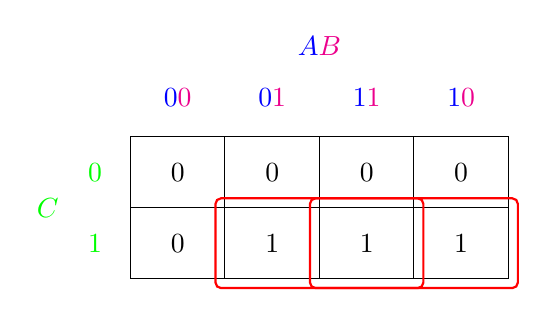
\begin{tikzpicture}[font=\normalsize]
  \draw (0,0) rectangle (4.8,-1.8);
  \draw (1.2,0) -- (1.2,-1.8);
  \draw (2.4,0) -- (2.4,-1.8);
  \draw (3.6,0) -- (3.6,-1.8);
  \draw (0,-0.9) -- (4.8,-0.9);
  \node at (0.6,-0.45) {0};
  \node at (1.8,-0.45) {0};
  \node at (3.0,-0.45) {0};
  \node at (4.2,-0.45) {0};
  \node at (0.6,-1.35) {0};
  \node at (1.8,-1.35) {1};
  \node at (3.0,-1.35) {1};
  \node at (4.2,-1.35) {1};
  \node at (0.6,0.5) {\textcolor{blue}{0}\textcolor{magenta}{0}};
  \node at (1.8,0.5) {\textcolor{blue}{0}\textcolor{magenta}{1}};
  \node at (3.0,0.5) {\textcolor{blue}{1}\textcolor{magenta}{1}};
  \node at (4.2,0.5) {\textcolor{blue}{1}\textcolor{magenta}{0}};
  \node at (2.4,1.15) {\textcolor{blue}{$A$}\textcolor{magenta}{$B$}};
  \node[text=green] at (-0.45,-0.45) {0};
  \node[text=green] at (-0.45,-1.35) {1};
  \node[text=green] at (-1.05,-0.9) {$C$};
  \draw[red, thick, rounded corners=2pt] (1.08,-0.78) rectangle (3.72,-1.92);
  \draw[red, thick, rounded corners=2pt] (2.28,-0.78) rectangle (4.92,-1.92);
\end{tikzpicture}
\end{center}
The two 1s in the row $C=1$ with $B=1$ (that is, $01$ and $11$) group to give $BC$, and the two 1s in the row $C=1$ with $A=1$ (that is, $11$ and $10$) group to give $AC$, so the K-map simplifies to $F=BC+AC$.\\\\
\textbf{Grouping conventions}
\begin{itemize}
    \item Groups must contain powers of 2: One, two, four, eight or sixteen 1s can be 
grouped together.
	\item Groups must be rectangular or square: Each group should form a rectangle or 
square shape. 
\item Groups cannot be diagonal: Adjacent 1s can only be grouped horizontally or vertically, 
not diagonally. 
\item Groups must be as large as possible: Always aim to make the largest groups to simplify the expression further. 
\item Groups can overlap: Some 1s may be included in more than one group if it helps form 
larger groups. 
\item Minimize the total number of groups: The goal is to use the smallest number of groups to cover all the 1s. 
    \end{itemize}
To determine the expression from the groups, we look at each group of cells and refer to the 
variables. If a variable’s value stays the same across all the cells in the group, we keep that 
variable in the simplified expression. Iowever, if the variable’s value changes across the group, we discard it from the expression. \\\\
\textbf{Wrapping around edges in K-maps}\\
K-maps are considered three-dimensional, and groups can be formed from left 
to right and top to bottom (although only left to right is possible with three inputs).
In the example of $F=\overline{B}+ABC$:
\begin{center}
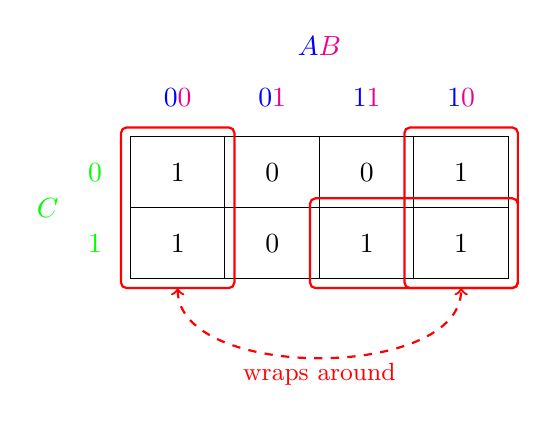
\begin{tikzpicture}[font=\normalsize]
  \draw (0,0) rectangle (4.8,-1.8);
  \draw (1.2,0) -- (1.2,-1.8);
  \draw (2.4,0) -- (2.4,-1.8);
  \draw (3.6,0) -- (3.6,-1.8);
  \draw (0,-0.9) -- (4.8,-0.9);
  \node at (0.6,-0.45) {1};
  \node at (1.8,-0.45) {0};
  \node at (3.0,-0.45) {0};
  \node at (4.2,-0.45) {1};
  \node at (0.6,-1.35) {1};
  \node at (1.8,-1.35) {0};
  \node at (3.0,-1.35) {1};
  \node at (4.2,-1.35) {1};
  \node at (0.6,0.5) {\textcolor{blue}{0}\textcolor{magenta}{0}};
  \node at (1.8,0.5) {\textcolor{blue}{0}\textcolor{magenta}{1}};
  \node at (3.0,0.5) {\textcolor{blue}{1}\textcolor{magenta}{1}};
  \node at (4.2,0.5) {\textcolor{blue}{1}\textcolor{magenta}{0}};
  \node at (2.4,1.15) {\textcolor{blue}{$A$}\textcolor{magenta}{$B$}};
  \node[text=green] at (-0.45,-0.45) {0};
  \node[text=green] at (-0.45,-1.35) {1};
  \node[text=green] at (-1.05,-0.9) {$C$};
  \draw[red, thick, rounded corners=2pt] (-0.12,0.12) rectangle (1.32,-1.92);
  \draw[red, thick, rounded corners=2pt] (3.48,0.12) rectangle (4.92,-1.92);
  \draw[red, thick, dashed, {<->}] (0.6,-1.92) .. controls (0.6,-3.1) and (4.2,-3.1) .. (4.2,-1.92);
  \node[red, font=\small] at (2.4,-3.02) {wraps around};
  \draw[red, thick, rounded corners=2pt] (2.28,-0.78) rectangle (4.92,-1.92);
\end{tikzpicture}
\end{center}
The four 1s in the columns $AB=00$ and $AB=10$ wrap around the left and right edges to form one group of four in which $B=0$ throughout, giving $\overline{B}$; the remaining 1 groups with the adjacent 1 in $AB=10$ (overlapping the $\overline{B}$ group) to give $AC$, so the K-map simplifies to $F=\overline{B}+AC$.
\\\\
Four-variable K-maps wrap in both directions, so the map behaves like a torus: the left and right edges join, and the top and bottom edges join as well. The figure shows a $4\times4$ map and the same map drawn on a torus; the four wrapping corner cells are marked with dots.
\begin{center}
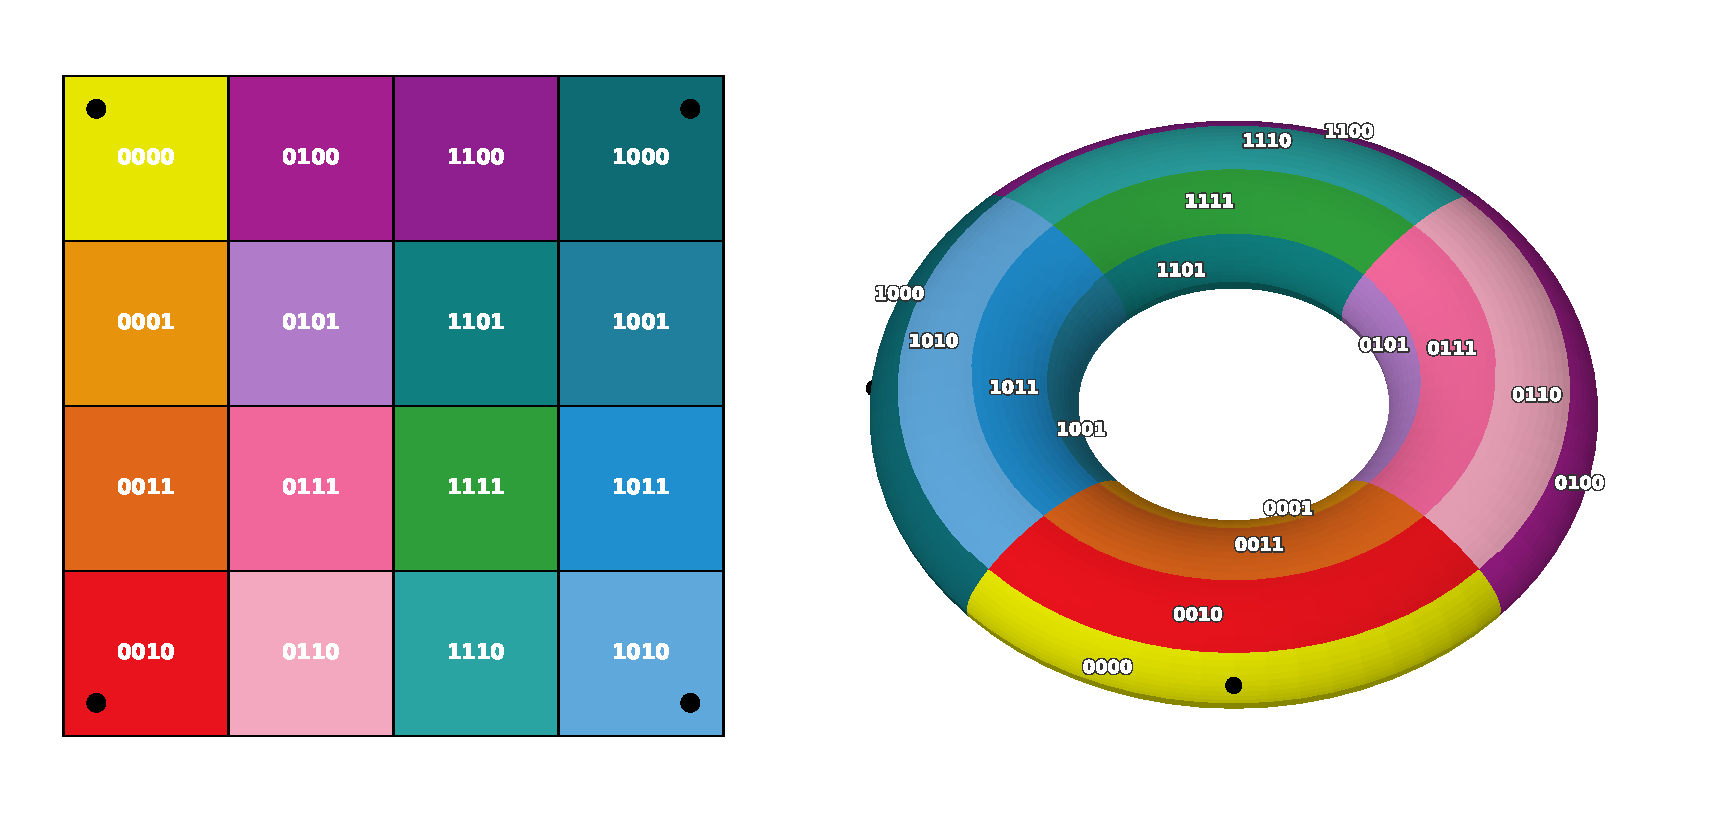
\includegraphics[width=0.95\linewidth]{kmap-torus.pdf}
\end{center}
\paragraph{Constructing logic diagrams}
By understanding the principles of Boolean algebra, we can simplify complex logic expressions and translate them into circuit diagrams. This journey from abstract mathematical notation 
to circuit design is essential for creating efficient and reliable digital systems. When a logic expression is given, follow the conventional operation sequence (parentheses first, then NOT, AND, OR...) 
\subsubsection{Operating systems and control systems}
\paragraph{The role of operating system}
An operating system (OS) is the fundamental software that manages computer hardware 
and software resources and provides common services for computer programs. It acts as an intermediary between the user and the computer hardware, ensuring efficient and secure operation of the system. Operating systems simplify user interactions with computer hardware by abstracting the underlying complexities (through providing a set of high-level services and interfaces).
\begin{itemize}
    \item CPU management: allocating CPU time to various processes and ensuring 
efficient execution 
	\item Memory management: handling the allocation and de-allocation of memory to 
applications, and managing virtual memory to extend physical memory capacity 
\item Storage management: organizing and managing data on storage devices, ensuring reliable data storage and retrieval 
\item Device management: controlling and co-ordinating hardware devices, providing drivers and interfaces for seamless operation. 
\end{itemize}
\paragraph{Functions of an operating system}
\begin{itemize}
    \item Memory management: control and coordination of a computer's primary memory; the OS ensures that memory is allocated efficiently to processes and applications, maintains system stability and protects memory areas from unauthorized access. When an app is opened, the OS will load it into RAM. How the memory allocation mechanism work:
    \begin{enumerate}
        \item Locate the app on the storage device and read the executable file, containing all the app's code and initial data. 
        \item The OS then allocates the necessary memory space for the application. This includes space for the code, data and any other required resources. The OS ensures that the application has enough space to execute without interfering with other processes. 
        \item Once the application is loaded into RAM, the OS continuously manages memory to ensure efficient operation and system stability.
        \begin{enumerate}
            \item While the application is running, the OS can dynamically allocate and de-allocate memory as needed by the application. 
            \item The OS also ensures that 
each process operates within its own memory space. This prevents processes from interfering with each other, which enhances the security and stability of the system. 
\item If the applications require more memory than is available in the RAM, the OS can use virtual memory to keep the system running smoothly. (Virtual Memory: a memory-management technique that allows a computer to use more memory than what's physically available by temporarily transferring data from RAM to disk storage, enabling the execution of larger programs and multitasking. )
            \end{enumerate}
    \end{enumerate}
    \item File management: involving the storage, retrieval, organization and manipulation of data on storage devices. The OS provides a structured way to manage files and directories, ensuring system stability and security. 
    \begin{enumerate}
        \item The OS employs a hierarchical file system to organize files in a logical and structured manner. Files are organized into directories (or folders), which can contain further directories, creating a tree-like structure. This organization makes it easier for users and applications to locate and manage data. 
        \item The OS allows a number of set file operations that users and applications can perform on the files and directories, including creating new files and directories; reading and writing data to files; deleting files; renaming files; and moving or copying files and directories to different locations. 
        \item To ensure consistency and avoid conflicts, the OS enforces rules for naming files, ensuring no two files in the same directory have the same name. Files often have extensions, like .jpg or .exe, to indicate the file type and associated application for opening these files.
        \item \textbf{Fragmentation} occurs over time as files are created, modified and deleted, causing them to be scattered across different sectors of the disk. Defragmentation aims to rearrange these file fragments into contiguous sequences, so improving system performance.
    \end{enumerate}
    \item Device management
    \begin{enumerate}
        \item The OS controls and co-ordinates the use of hardware components such as printers, disk drives, display screens, keyboards and network interfaces through specialized software called device drivers. (specialized software programs that allow the operating system to communicate with and control hardware devices, e.g. printers, graphics cards or network adapters, by providing 
the necessary instructions and protocols. )
	\item The OS also handles input/output (I/0) management to co-ordinate data transfer between the computer and peripheral devices. It employs techniques such as buffering, caching and spooling to optimize performance and reliability.
	\begin{enumerate}
	    \item Buffering: the process of temporarily storing data in a memory area (buffer) while it is being transferred between two devices or processes, helping to manage differences in data-flow rates and ensuring smooth, uninterrupted operation.
	    \item Caching: the process of temporarily storing frequently accessed data in a high-speed storage area (cache) to reduce access time and improve system performance by enabling quicker retrieval of the data. 
	    \item Spooling: the process of gqueuing data or tasks in a buffer, typically for input / output devices such as printers, so that they can be processed sequentially and at their own pace, allowing the system to continue working on other tasks in the meantime.
	    \end{enumerate}
\item Modern operating systems have introduced user-friendly ways of connecting devices, such as Plug and Play (PnP) technology. With PnP, the OS can automatically identify a device that has been attached and install the necessary drivers and configure settings without the need for user interaction. The OS is also capable of detecting errors and taking action to recover from them, by resetting the device, reinitializing drivers or notifying the user of the issue. Additionally, the OS provides security and access control to ensure that only authorized users and processes can access certain devices, maintaining system integrity and security. 
    \end{enumerate}
\begin{center}
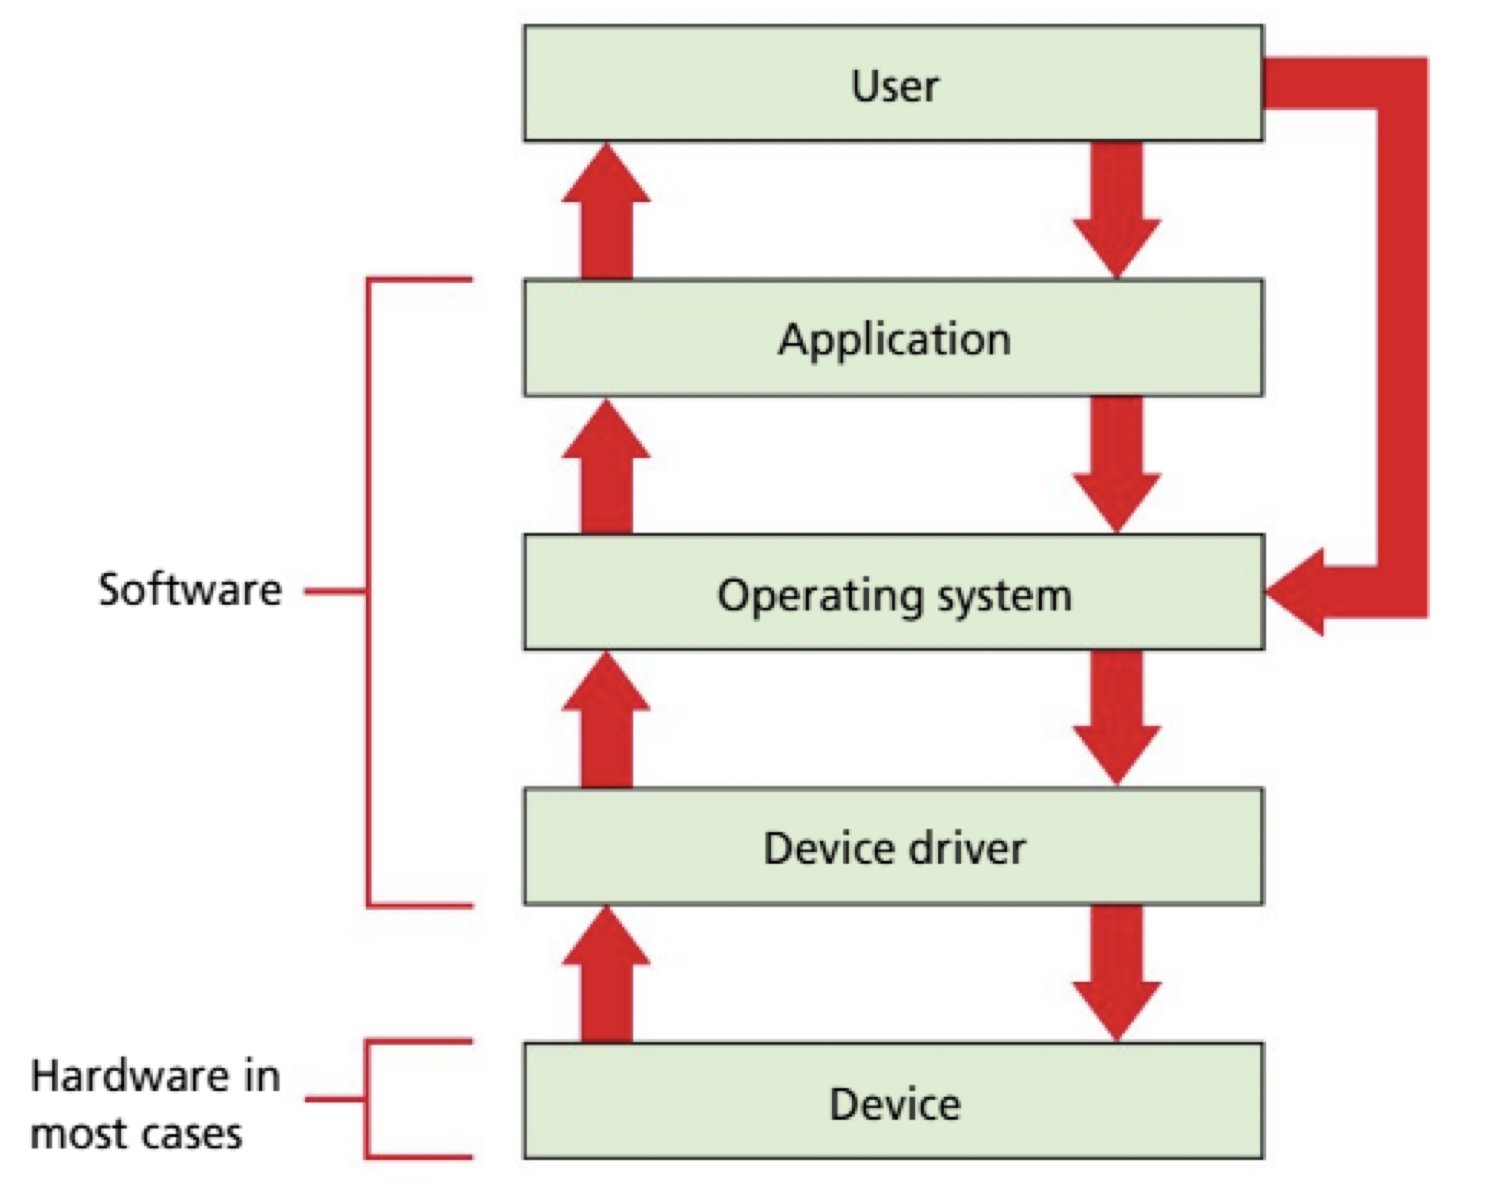
\includegraphics[width=0.6\linewidth]{Screenshot 2026-10-19 at 18.51.25.png}
\end{center}
    \item Scheduling: The OS schedules the process of managing the execution of multiple processes by determining which process runs at any given time. The scheduler is responsible for allocating CPU time to processes, ensuring efficient and fair use of system resources. This function is crucial for mulritasking environments, where multiple applications and background processes run concurrently. By implementing various scheduling algorithms, the OS aims to optimize performance, reduce wait times and maintain system stabiliry. 
    \item Security
    \begin{itemize}
        \item User authentication
        \item Encryption
        \item Auditing and monitoring
        \item Malware protection
        \end{itemize}
    \item Accounting
    \begin{itemize}
        \item Resource usage tracking
        \item Process accounting
        \item User accounting
        \item Performance monitoring
        \item Auditing and reporting
        \item Billing and chargeback
        \end{itemize}
    \item GUI: By offering visual elements such as windows, icons, menus and pointers, the OS provides a user-friendly environment for interacting with the computer and allows the user to execure commands, manage files and run applications. 
    \begin{itemize}
        \item User interface elements
        \item Application management
        \item File and system management
        \item Accessibility
        \item Visual feedback
        \item Customization and personalization
        \end{itemize}
    \item Virtualization
    \item Networking
\end{itemize}
\paragraph{Approaches for scheduling}
An operaring system needs scheduling methods to efficiently manage the execution of multiple processes, ensuring optimal use of the CPU and other resources. Without effective scheduling, processes could experience significant delays or monopolize resources (domination of system resources by a single process, reducing available resources for other processes, thereby slowing system down / inefficiency)
\begin{itemize}
    \item First Come First Served, FCFS
    \item Round Robin, RR
    \item Priority Scheduling
    \item Multilevel Queue Scheduling
    \item (Shortest-Job First)
\end{itemize}
\paragraph{Interrupt handling and polling}
\paragraph{The role of the operating system in managing multitasking and resource allocation}
\paragraph{The use of system components}
\paragraph{The uses of control systems}
\subsubsection{Translation}
\subsection{Networks}
\subsubsection{Network fundamentals}
\subsubsection{Network architecture}
\subsubsection{Data transmission}
\subsubsection{Network security}
\subsection{Databases}
\subsubsection{Database fundamentals}
\subsubsection{Database design}
\subsubsection{Database programming}
\subsubsection{Alternative databases and data warehouses}
\subsection{Machine learning}
\subsubsection{Machine learning fundamentals}
\subsubsection{Data preprocessing}
\subsubsection{Machine learning approaches}
\subsubsection{Ethical considerations}

\newpage
\section{Computational Thinking and Problem Solving}
\subsection{Computational thinking}
\subsubsection{Approaches to computational thinking}
\paragraph{Problem specification}
\paragraph{Fundamental concepts of computational thinking}
\begin{itemize}
    \item Abstraction
    \begin{itemize}
        \item Definition: the process of extracting essential information, while disregarding irrelevant data, to propose or outline a feasible solution to a given problem.
        \item Why it is important: Hide complexity from the user by abstracting data entities and hiding underlying implementation of a process.
        \item By using abstraction: the time required to create a piece of software is reduced; the program becomes smaller in size, so it requires less space in memory and the download times are reduced; customer satisfaction increases, as their requirements are met without extra features. 
    \end{itemize}
\end{itemize}

\subsection{Programming}
\subsubsection{Programming fundamentals}
\subsubsection{Programming constructs}
\subsubsection{Data structures}
\subsubsection{Programming algorithms}
\subsubsection{File processing}
\subsection{Object-oriented programming (OOP)}
\subsubsection{Fundamentals of OOP for a single class}
\subsubsection{Fundamentals of OOP for multiple classes}
\subsection{Abstract data types (ADTs)}
\subsubsection{Fundamentals of abstract data types}
\newpage
\section{Appendices}
\subsubsection{My favourite operating system: Arch Linux (+ Hyprland)}
\paragraph{What it is}
Arch Linux is a lightweight, rolling-release distribution built around the principle of user-centricity: you start from a minimal base and build up exactly the system you want, installing only the packages you actually need. On top of it I run Hyprland, a dynamic tiling Wayland compositor, which handles all the window management and visual effects. Together they are not a finished product you install, but a system you assemble and shape yourself.
\paragraph{Why it is my favourite}
\begin{itemize}
    \item Customizability: nothing is assumed for me. Every package, service, kernel module and keybind is a deliberate choice, so the OS fits my workflow instead of the other way around. Hyprland is configured entirely through a plain-text file, so layouts, animations and rules can be tuned down to the pixel.
    \item Responsiveness and performance: the system ships with no bundled bloatware or background services, so boot times are short and idle resource usage is very low. On the same hardware, a minimal Arch + Hyprland setup feels noticeably snappier than a stock desktop environment.
    \item Rolling release: packages are updated continuously rather than frozen until the next major version, so I always have current kernels, drivers and toolchains without a disruptive reinstall.
    \item The AUR and community: the Arch User Repository gives access to an enormous range of community-maintained packages, and the Arch Wiki is arguably the best-documented Linux resource available, which makes troubleshooting a learning exercise rather than a dead end.
    \item Keyboard-driven workflow: as a tiling compositor, Hyprland automatically arranges windows with no manual dragging, which keeps my hands on the keyboard, reduces context switching and makes multitasking far faster.
    \item Learning and control: because I built the system, I understand how each layer fits together. Using Arch teaches real operating-system concepts — package management, the boot process, display servers, resource allocation — which connects directly back to the OS material in Section A.
\end{itemize}
A rolling-release, build-it-yourself system does come with trade-offs: upgrades occasionally break things and demand manual intervention, and there is no vendor support to fall back on. For me that trade-off is worth it — the control and understanding I gain outweigh the convenience I give up.

\end{document}
